\documentclass[5p,times]{elsarticle}
%===============
\usepackage[colorlinks=true,allcolors=blue]{hyperref}
\usepackage{graphicx}

\usepackage{epstopdf}
\usepackage{dcolumn}
\usepackage{bm}
%\usepackage[mathlines]{lineno}
%\linenumbers\relax

\usepackage{xr-hyper}
%\externaldocument{ITIC-supp}
%\externaldocument[S-]{ITIC-supp}


\usepackage[latin1]{inputenc}
\usepackage{tikz}
\usetikzlibrary{shapes,arrows}

%\usepackage{enumitem}

\usepackage[position=top]{subfig}


%===============
\usepackage{lineno,hyperref}

\modulolinenumbers[5]

\journal{Fluid Phase Equilibria}

%%%%%%%%%%%%%%%%%%%%%%%
%% Elsevier bibliography styles
%%%%%%%%%%%%%%%%%%%%%%%
%% To change the style, put a % in front of the second line of the current style and
%% remove the % from the second line of the style you would like to use.
%%%%%%%%%%%%%%%%%%%%%%%

%% Numbered
%\bibliographystyle{model1-num-names}

%% Numbered without titles
%\bibliographystyle{model1a-num-names}

%% Harvard
%\bibliographystyle{model2-names.bst}\biboptions{authoryear}

%% Vancouver numbered
%\usepackage{numcompress}\bibliographystyle{model3-num-names}

%% Vancouver name/year
%\usepackage{numcompress}\bibliographystyle{model4-names}\biboptions{authoryear}

%% APA style
%\bibliographystyle{model5-names}\biboptions{authoryear}

%% AMA style
%\usepackage{numcompress}\bibliographystyle{model6-num-names}

%% `Elsevier LaTeX' style
\bibliographystyle{elsarticle-num}
%%%%%%%%%%%%%%%%%%%%%%%
\hypersetup{draft}
\begin{document}

\begin{frontmatter}

\title{Coexistence Calculation Using the Isothermal-Isochoric Integration Method}

%% Group authors per affiliation:
\author{S. Mostafa Razavi}
\ead{sr87@uakron.edu}
\address{Department of Chemical and Biomolecular Engineering, The University of Akron, Akron, Ohio 44325, USA}

\author{Richard A. Messerly}
\ead{richard.messerly@nist.gov}
\address{Thermodynamics Research Center, National Institute of Standards and Technology, Boulder, Colorado 80305, USA}

%% or include affiliations in footnotes:
%\author[mymainaddress,mysecondaryaddress]{Elsevier Inc}
%\ead[url]{www.elsevier.com}


\author{J. Richard Elliott \corref{mycorrespondingauthor}}
\cortext[mycorrespondingauthor]{Corresponding author}
\ead{elliot1@uakron.edu}
\address{Department of Chemical and Biomolecular Engineering, The University of Akron, Akron, Ohio 44325, USA}

\begin{abstract}
In this work, the isothermal-isochoric integration (ITIC) method is demonstrated as a viable method for vapor-liquid coexistence calculation by molecular simulation. Several tests are carried out to validate the method which results in less than 1 \% deviation from NIST REFPROP values for reduced temperatures of less than 0.85. Consistency is achieved between the ITIC method, Gibbs Ensemble Monte Carlo (GEMC) method, and Grand Canonical Monte Carlo (GCMC) method for reduced temperatures of 0.6-0.85. The ITIC method proves to be much more effective compared to GEMC and GCMC methods for vapor-liquid coexistence calculations at reduced temperatures of 0.45-0.6, where relative deviations from experimental data are often quite large but important for practical applications. It is shown that computational efficiency is often served best by applying the ITIC method for the entire temperature range rather than applying Monte Carlo (MC) methods for part of the range. Furthermore, the ITIC method lends itself to application with molecular dynamics (MD) as well as MC, advancing the prospect of simulation results that are quantitatively consistent across software platforms.
\end{abstract}

\begin{keyword}
Vapor Pressure, Vapor Liquid Equilibria, Phase Diagram, Liquid Density
\end{keyword}

\end{frontmatter}

%\linenumbers

\section{Introduction} \label{sec:introduction}
Phase coexistence determination is important when characterizing the physical properties of a chemical compound. Both the vapor pressure ($P^{\mathrm{sat}}$) and saturation liquid and vapor density ($\rho_{\mathrm{liq}}$ and $\rho_{\mathrm{vap}}$) provide sensitive measures of the quality provided by a particular force field. In principle, the computation of phase coexistence is a simple matter of equating pressures, temperatures, and chemical potentials between the coexisting phases. Nevertheless, accurate computation of phase coexistence by molecular simulation has posed challenges over the years. 

The most straightforward method to compute phase transition in molecular simulation is to simply define an $NVT$ system (constant number of molecules, volume, and temperature) of sufficient size and overall density that an explicit interface is encountered. However this method often results in imprecise results \cite{Frenkel1996}. First order phase transitions exhibit a considerable free energy barrier between two phases due to interfacial free energies. For systems with large interfaces, this energy barrier increases. This often results in hysteresis, and phase transformation irreversibly proceeds beyond the coexistence point. \cite{Frenkel1996} 

Alternatively, there are methods for calculating phase coexistence while avoiding explicit interfaces. The Gibbs Ensemble Monte Carlo (GEMC) method \cite{Panagiotopoulos1987} is one of the most popular phase coexistence determination methods \cite{Paluch2008}.  GEMC requires particle exchange between two phases which leads to its major drawback, i.e. insertion of particles in dense phases for large molecules. Histogram reweighting Monte Carlo and Transition-matrix Monte Carlo methods 
are two closely related methods used for calculation of phase equilibrium based on Grand Canonical Monte Carlo (GCMC) simulations. These methods also involve the problematic insertion/deletion moves. This problem is especially exacerbated  at low temperatures and for large and branched molecules. The lowest temperatures that are available in the literature rarely extend below a reduced temperature ($T_\mathrm{r} = T/T_\mathrm{c}$, where $T_\mathrm{c}$ is the critical temperature) of 0.6 \cite{Martin1998,Potoff2009}. However, common methods for industrial applications treat the temperature range from triple point to the critical point. The Peng-Robinson equation of state, for example, is valid for reduced temperatures as low as 0.45 \cite{Peng1976}. To provide fundamental physical models that address issues with industrial applications, molecular simulations must address the entire temperature range of interest. 

As another alternative, Kofke \cite{Kofke1993b} developed a method called Gibbs-Duhem integration which makes use of the Clapeyron equation to numerically integrate and proceed along the saturation line starting from one single coexistence point. The Gibbs-Duhem method can solve the insertion problem, but it relies on a second method to obtain the initial coexistence point. Ahunbay et al. \cite{Ahunbay2004} have applied this approach in conjunction with GEMC 
to obtain the initial coexistence point, $NPT$ simulations to estimate saturation liquid densities, and parallel tempering method \cite{Yan1999} to increase the efficiency of low temperature simulations. Their implementation is tested at reduced temperatures above 0.45 for several compounds. Note that in Gibbs-Duhem method, vapor density can also be obtained from the ideal gas equation or through separate $NPT$ simulations at the computed saturation pressure and temperature.

%Ahunbay et al. \cite{Ahunbay2004} have applied this approach in conjunction with GEMC to obtain the initial coexistence point, $NPT$ simulations to estimate saturation liquid densities, and parallel tempering method \cite{Yan1999} to increase the efficiency of low temperature simulations. Their implementation is tested at reduced temperatures above 0.45 for several compounds, however it does not provide saturation vapor density unless it is calculated directly from GEMC simulation.

As one more alternative, thermodynamic integration can provide a reliable solution for free energy calculation. In this method, a series of simulations are performed along a path that connects the state of interest to a system for which the free energy is known. One should be careful that the path does not include any type of phase change\cite{Vega2009}. Elliott et al. \cite{Elliott1999a} applied an isochoric integration method to calculate vapor-liquid equilibria (VLE) of square well spheres, demonstrating deficiencies in the preceding MC results.  For square well spheres, a convenient starting isotherm is the hard sphere limit, for which the thermodynamics are well represented by the Carnahan-Starling equation\cite{Carnahan1969a}. In this work, however, results are sought for soft potential models of arbitrary molecular shape, for which the infinite temperature limit is not convenient. 

In the proposed method, $NVT$ simulation points are used across an isotherm and along several isochores, hence the name isothermal-isochoric (ITIC). Because the approach to low temperatures proceeds along an isochore initialized at the high temperature (supercritical) isotherm, the insertion move problem is alleviated. In principle, there is no low temperature limit for the applicability of this method, except the triple point. Also, the data generated along the paths of integration are valuable on their own merits, providing distinct insights about how well the molecular model is performing under conditions of high temperature and pressure. In other words, ITIC provides greater quality of characterization than other vapor-liquid coexistence calculations at low saturation temperatures and non-saturation temperatures. In addition, with combination of derivative properties from the work of Lustig et al \cite{Lustig2015}, it should be possible to utilize this data in order to generate high accuracy multi-parameter equations of states, similar to the work of Thol et al. \cite{Thol2015b} for LJ spheres.

As another advantage, vapor pressure calculation using molecular dynamics (MD) is often perceived as an impractical approach \cite{Nieto-Draghi2015}. In this work, we show the possibility of using molecular dynamics in the context of ITIC integration as a viable tool for VLE calculation. The ITIC method provides a cross-platform solution to the problem of VLE calculation without a significant increase in computational effort compared to the typical GEMC or GCMC approaches.
 
The presentation is initiated in Section~\ref{sec:ITIC-method} with a review of the thermodynamics underlying the integration method and some practical implementation aspects. The approach is validated in Section~\ref{sec:NIST-VAL} by applying it to coexistence data available from the National Institute of Standards and Technology (NIST). Section~\ref{sec:SimDetail} describes the details of simulations that are found in Sections~\ref{sec:VirialCalc}-\ref{sec:ExampleSim}. Section~\ref{sec:VirialCalc} provides recommendations for the most convenient and effective methods for characterizing the virial coefficients by molecular simulation. Section~\ref{sec:FSE} investigates the magnitude of finite size effects. Section~\ref{sec:ExampleSim} demonstrates applications to molecular simulations and comparison between the ITIC method and other methods of phase coexistence calculation. Finally, Section~\ref{sec:conclusion} summarizes the conclusions from this work.

\section{The Isothermal-Isochoric Integration Method} \label{sec:ITIC-method}
\subsection{Free energy departure function derivation}
For a single component system, Eq.~(\ref{eqn:eqn1}) must be satisfied at vapor-liquid phase equilibrium
\begin{equation}
\begin{array}{l}
{T_\mathrm{vap} =T_\mathrm{liq} }\\
{P_\mathrm{vap} =P_\mathrm{liq} }\\
{G_\mathrm{vap} =G_\mathrm{liq} }
\end{array} 
\label{eqn:eqn1}
\end{equation}
where $G$ represents the molar Gibbs free energy, $T$ is the temperature, $P$ is pressure, and subscripts ``vap" and ``liq" denote the vapor and liquid phases, respectively. 

The Gibbs energy criterion of phase equilibrium can be rewritten in departure function form

\begin{equation}
\left(\frac{G_\mathrm{liq} -G_\mathrm{ig} }{RT}\right)_{T,P} =\left(\frac{G_\mathrm{vap}-G_\mathrm{ig}}{RT}\right)_{T,P} \label{eqn:eqn9}
\end{equation}
where the subscript ``ig" denotes the ideal gas, and $R$ is the gas constant ($8.3144598\,\mathrm{J/(mol\,K)}$). This equation can be rearranged in terms of the Helmholtz energy ($A$) departure function 
\begin{equation}
\begin{array}{l}
{\left(\frac{A_\mathrm{liq} -A_\mathrm{ig} }{RT} \right)_{T,V} +Z_{\mathrm{liq}} -1-\ln(Z_{\mathrm{liq}})} 
\\ 
{=\left(\frac{A_\mathrm{vap} -A_\mathrm{ig} }{RT} \right)_{T,V} +Z_{\mathrm{vap}} -1-\ln(Z_{\mathrm{vap}})}  
\end{array} 
\label{eqn:eqn10}
\end{equation}
where $Z$ is the compressibility factor $(Z \equiv \frac{P}{\rho RT})$. Note that the $\ln(Z)$ terms are introduced when converting Gibbs energy departure function at constant $T,P$ in Eq.~(\ref{eqn:eqn9}) to Helmholtz energy departure function at constant $T,V$ in Eq.~(\ref{eqn:eqn10}) \cite{Elliott1999}. Calculating free energy of a system using the ITIC integration method involves connecting the state of interest to a state of known free energy. In the case of phase equilibrium calculation, the state of interest is saturated liquid and the state of known free energy is an ideal gas. In order to connect saturated liquid to low densities we cannot cross the two phase region. Instead, the temperature of saturated liquid is increased to a supercritical temperature through an isochoric path, then the supercritical state is connected to low densities through an isothermal path. Several separate simulations in the canonical ensemble ($NVT$) are needed to provide enough data points on the paths for numerical integration to be accurate. 

The first stage involves integrating internal energy, $U$, according to Eq.~(\ref{eqn:eqn6}) which is derived using Eqs.~(\ref{eqn:eqn2}-\ref{eqn:eqn5}). Eq.~(\ref{eqn:eqn6}) is obtained from Eq.~(\ref{eqn:eqn5}) by taking the difference between the real and ideal gas states (where the constants of integration cancel). 

\begin{equation}
U=kT^{2} \left( \frac{\partial \ln Q}{\partial T}\right) _{N,V}  \label{eqn:eqn2}
\end{equation}

\begin{equation}
A \left( N,V,T \right)=-kT \ln Q\left(N,V,T\right)
\label{eqn:eqn3}
\end{equation}

\begin{equation}
U=kT^{2} \left( \frac{\partial (-A/kT)}{\partial T} \right)_{N,V} =\frac{\partial \beta A}{\partial \beta }  \label{eqn:eqn4}
\end{equation}

\begin{equation}
\beta A=\int U\mathrm{d} \beta + \mathrm{constant}  \label{eqn:eqn5}
\end{equation}

\begin{equation}
 \frac{A-A_\mathrm{ig} }{RT} =\int \frac{U-U_\mathrm{ig}}{R} \mathrm{d}\left( \frac{1}{T} \right) \label{eqn:eqn6}
\end{equation}
where $V$ represents volume,  $k$ is the Boltzmann constant, $\beta \equiv \frac{1}{kT}$, and $Q$ is the canonical partition function.


The second stage consists in performing the following integration
\begin{equation}
\frac{A-A_\mathrm{ig}}{RT} =\; \int _{0}^{\rho }\frac{Z-1}{\rho } \; \mathrm{d}\rho \label{eqn:eqn7}
\end{equation}
where $\rho$ represents density.

Therefore, the Helmholtz energy departure function of the liquid phase is calculated using Eq.~(\ref{eqn:eqn8})

\begin{equation}
\begingroup
\large
\begin{array}{l}
\left( \frac{A_\mathrm{liq} -A_\mathrm{ig} }{RT} \right)_{T,V}
\\ 
{=\; \int _{0}^{\rho _{\mathrm{liq}} }\frac{Z-1}{\rho } \; \mathrm{d}\rho \mathop{|}\nolimits_{T^{\mathrm{IT}}} +\int _{T^{\mathrm{IT}}}^{T^{\mathrm{\mathrm{sat}}}
} \frac{U-U_\mathrm{ig}}{R} \; \mathrm{d} \left(\frac{1}{T} \right) \mathop{|}\nolimits_{\rho _{\mathrm{liq}}}}  
\end{array} 
\endgroup
\label{eqn:eqn8}
\end{equation}
where the first integral is performed along the supercritical isotherm ($T^{\mathrm{IT}} \approx 1.2\,T_\mathrm{c}$) from zero density to the saturated liquid density of interest, and second integral is performed along the saturated liquid density isochore from $T_\mathrm{r} \approx 1.2$ to saturation temperature $T^\mathrm{sat}$.

The value for $Z_{\mathrm{vap}}$ in Eq.~(\ref{eqn:eqn10}) can be approximated using a virial expansion truncated at the $B_3$ term, because the density of vapor phase is low at most conditions of interest.

\begin{equation}
{Z_{\mathrm{vap}}} = 1 + {B_2}{\rho_{\mathrm{vap}}} + {B_3}\rho_{\mathrm{vap}}^2
\label{eqn:eqn11}
\end{equation}
which is substituted in Eq.~(\ref{eqn:eqn7}) to obtain free energy departure function of vapor phase

\begin{equation}
\begingroup
\large
\begin{array}{l}{\left( {\frac{{{A_\mathrm{vap}} - {A_\mathrm{ig}}}}{{RT}}} \right)_{T,V}} = \int_0^{{\rho _{\mathrm{vap}}}} {\frac{{Z - 1}}{\rho } \mathrm{d}\rho } \\ = \int_0^{{\rho
_{\mathrm{vap}}}} {\frac{{{B_2}{\rho _{\mathrm{vap}}} + {B_3}\rho _{\mathrm{vap}}^2}}{\rho_{\mathrm{vap}} } \mathrm{d}\rho_{\mathrm{vap}} } = {B_2}{\rho _{\mathrm{vap}}} + \frac{1}{2}{B_3}\rho _{\mathrm{vap}}^2\end{array} 
\endgroup
\label{eqn:eqn12}
\end{equation}

\subsection{Vapor pressure and density calculation}
We have characterized the Helmholtz energy departure function in vapor and liquid phases. Substituting Eq.~(\ref{eqn:eqn8}) and Eq.~(\ref{eqn:eqn12}) in Eq.~(\ref{eqn:eqn10}) yields

\begin{equation}
\left( \frac{ A_\mathrm{liq} - A_\mathrm{ig} }{{RT}} \right)_{T,V} + {Z_{\mathrm{liq}}} - 1 + \ln \left( \frac{{{\rho _{\mathrm{liq}}}}}{{{\rho _{\mathrm{vap}}}}} \right) = 2{B_2} {\rho _{\mathrm{vap}}} + \frac{3}{2}{B_3} \rho _{\mathrm{vap}}^2 \label{eqn:eqn14}
\end{equation}
which can be rearranged in terms of ${\rho_\mathrm{vap}}$ 

\begin{equation}
\begin{array}{l}
{\rho _{\mathrm{vap}} = }
\\ 
{{\rho _{\mathrm{liq}}}\exp \left( {{{\left( {\frac{{{A_\mathrm{liq}} - {A_\mathrm{ig}}}}{{RT}}} \right)}_{T,V}} + {Z_{\mathrm{liq}}} - 1 - 2{B_2} {\rho _{\mathrm{vap}}} - \frac{3}{2}{B_3} \rho _{\mathrm{vap}}^2}
\right) }  
\end{array}
\label{eqn:rhoV}
\end{equation}

Eq.~(\ref{eqn:rhoV}) can be solved for $\rho_\mathrm{vap}$ using the fixed-point iteration method \cite{Burden1985}. For simplicity, we solve this equation with the fixed-point iteration method. Finally, vapor pressure is calculated using Eq.~(\ref{eqn:psat})

\begin{equation}
P^\mathrm{sat} = P_\mathrm{vap} = {Z_\mathrm{vap}}{\rho _\mathrm{vap}}RT^\mathrm{sat} = (1 + {B_2} {\rho_\mathrm{vap}} + {B_3}\rho _\mathrm{vap}^2){\rho _\mathrm{vap}}RT^\mathrm{sat} 
\label{eqn:psat}
\end{equation}



\subsection{ITIC algorithm}
Implementation of the ITIC procedure starts with determining the temperatures and densities of the ITIC points shown in Figure~\ref{fig:ITICpathway}. In ITIC method, $\rho_\mathrm{liq}$ is imposed and $T^\mathrm{sat}$, $P^\mathrm{sat}$, and $\rho_\mathrm{liq}$ are calculated. This involves estimating saturation temperatures ($T^\mathrm{sat}_\mathrm{est}$), i.e. $T$ at points 11, 13, 15, 17, and 19. Once ITIC state points are determined, $NVT$ simulations are performed at the obtained conditions using either MD or MC, and the ensemble averages of compressibility factor and internal energy departure function ($U^\mathrm{dep}=\frac{U-U_\mathrm{ig}}{RT}$) are calculated from simulation output. Helmholtz energy departure function ($A^\mathrm{dep}$) is then calculated as explained in Section~\ref{sec:ITIC-state-points}, i.e. Eq~(\ref{eqn:eqn18}-\ref{eqn:eqn19}). At this point, $T^\mathrm{sat}$, $\rho_\mathrm{vap}$, and $P^\mathrm{sat}$ are solved iteratively for each isochore. First, $\rho_\mathrm{vap}$ and $Z_\mathrm{liq}$ are set to an initial near-zero value. Then, $\rho_\mathrm{vap}$ and $P^\mathrm{sat}$ are recomputed using Eq.~(\ref{eqn:rhoV}) and Eq.~(\ref{eqn:psat}), respectively. Then, $Z_\mathrm{liq}$ is updated as 
\begin{equation}
{Z_{\mathrm{liq}}} = \frac{P^\mathrm{sat}}{\rho_\mathrm{liq}RT^\mathrm{sat}}  
\label{eqn:zliq}
\end{equation}
where $\rho_\mathrm{liq}$ is equal to the isochoric density.

Next, $T^\mathrm{sat}$ is updated by inter- or extrapolating the isochoric simulation results, specifically, we fit Z vs reciprocal temperature to a second order polynomial and solve for Tsat such that $Z(T^\mathrm{sat})=Z_\mathrm{liq}$. 
%Next, $T^\mathrm{sat}$ is updated by inter- or extrapolating $Z$ vs reciprocal temperature along the isochore, using second order polynomial scheme, such that $Z(T^\mathrm{sat})=Z_\mathrm{liq}$. 
Since the value of $T^\mathrm{sat}$ has changed, $A^\mathrm{dep}$ should also be recomputed. Trapezoid rule is used to integrate $U^\mathrm{dep}T$ vs. $1/T$ (i.e. $(U-U^\mathrm{ig})/R$ vs. $1/T$ in Eq.~\ref{eqn:eqn6}) due to the linear shape of $U^\mathrm{dep}T$ vs. $1/T$ in the vicinity of $T^\mathrm{sat}$.

\begin{equation}
A^\mathrm{dep}_\mathrm{new} = A^\mathrm{dep}_\mathrm{old} + \left( \frac{1}{T^\mathrm{sat}_\mathrm{new}}-\frac{1}{T^\mathrm{sat}_\mathrm{old}} \right) \frac{U^\mathrm{dep}_\mathrm{new}T^\mathrm{sat}_\mathrm{new}+U^\mathrm{dep}_\mathrm{old}T^\mathrm{sat}_\mathrm{old}}{2} 
\label{eqn:aDepCorrection}
\end{equation}
where subscript ``old" denotes the corresponding property at $T^\mathrm{sat}_\mathrm{old}$ and subscript ``new" denotes the property at updated $T^\mathrm{sat}_\mathrm{new}$ (For the first iteration, $T^\mathrm{sat}_\mathrm{old} = T^\mathrm{sat}_\mathrm{est}$). Note that $U^\mathrm{dep}_\mathrm{new}$ is calculated by inter- or extrapolating $U^\mathrm{dep}$ vs $1000/T$ along the isochore, i.e., $U^\mathrm{dep}_\mathrm{new} = U^\mathrm{dep}(T^\mathrm{sat}_\mathrm{new})$.

Having new values for $T^\mathrm{sat}$, $Z_{\mathrm{liq}}$, $\rho_\mathrm{vap}$, and $A^\mathrm{dep}$ the next iteration starts from Eq.~(\ref{eqn:rhoV}). The iterations are stopped when the difference in two consecutive $\rho_\mathrm{vap}$ (or $T^\mathrm{sat}$) values are less than a defined tolerance (We use 0.1 \% deviation as the stopping criterion. Using smaller tolerances does not significantly improve the accuracy.) This procedure is repeated for other isochores. Figure~2 illustrates a detailed step-by-step algorithm starting from determining ITIC state points to obtaining VLE properties. This algorithm also includes a step for obtaining second virial coefficient along isotherm ($B_2^\mathrm{IT}$) and saturation second virial coefficients ($B_2^\mathrm{sat}$) which is explained in Section~\ref{sec:VirialCalc}.
\begin{figure}
\includegraphics[scale=0.45]{Figures/ITIC-pathway-C2-2.png}
\caption{A schematic plot of the pathways taken in the ITIC method. The y-axis represents the reciprocal reduced temperature and the x-axis shows the reduced density. Squares and diamonds represent non-saturated state points obtained from simulation, while orange and red circles represent liquid and vapor side of coexistence points calculated using the ITIC method. Green and purple diamonds show the state points required for $B_2$ calculation at isothermal temperature and $T_\mathrm{r}=0.9$, respectively. Note that square points 11, 13, 15, 17, and 19 represent the initial estimate of saturation temperature, therefore they do not necessarily match the coexistence curve.}
\label{fig:ITICpathway}
\end{figure}

\begin{figure}[]
\centering
\tikzstyle{decision} = [diamond, draw, fill=blue!20, text width=6em, text badly centered, node distance=2cm, inner sep=0pt]
\tikzstyle{block} = [rectangle, draw, fill=blue!20, text width=20em, text centered, rounded corners, minimum height=1em]
\tikzstyle{block22} = [rectangle, draw, fill=blue!20, text width=19em, text centered, rounded corners, minimum height=1em]
\tikzstyle{block15} = [rectangle, draw, fill=blue!20, text width=15em, text centered, rounded corners, minimum height=1em]
\tikzstyle{smallblock} = [rectangle, draw, fill=blue!20, text width=8em, text centered, rounded corners, minimum height=1em]
\tikzstyle{line} = [draw, -latex']

\begin{tikzpicture}[node distance = 1cm, auto,thick,scale=0.8, every node/.style={scale=0.8}]
\node [block22] (pre1) {
\footnotesize Determine $\rho$ and $T$ values in Figure~\ref{fig:ITICpathway}:
\begin{itemize}[]
\item \footnotesize Choose $\rho^9$, and calculate $\rho^{1-8}$
\item \footnotesize Estimate $T^\mathrm{sat}_\mathrm{est}$ values ($T^{11,13,15,17,19}$)
\item \footnotesize Calculate $T^{10,12,14,16,18}$
\item \footnotesize Choose $\rho$ for diamond points ($T_\mathrm{IT}$ and $T_\mathrm{0.9}$ isotherms)
\end{itemize}
};

\node [smallblock, below of=pre1,node distance=2.2cm] (step1) {\footnotesize Run $NVT$ simulations};
\node [block,below of=step1,node distance=1cm] (step2) {\footnotesize Calculate $Z$, $U^\mathrm{dep}$ for all $NVT$ simulations};
\node [block,below of=step2,node distance=1cm] (stepstep) {\footnotesize Calculate $B_2^\mathrm{IT}$ (Eq.~\ref{eqn:Z1rhoB2B3}) and $B_2^\mathrm{sat}$ correlation (Section~\ref{sec:VirialCalc})};
\node [block,below of=stepstep,node distance=1cm] (step5) {\footnotesize For each IC, calculate $A^\mathrm{dep}$ based on $T^\mathrm{sat}=T^\mathrm{sat}_\mathrm{est}$ (Eq.~\ref{eqn:eqn8})};
\node [block,below of=step5,node distance=2cm] (step4) {\footnotesize Calculate $T^\mathrm{sat}_\mathrm{new}$ from $Z$ vs. $1/T$  such that $Z(T^\mathrm{sat}) = Z_\mathrm{liq}$ };
\node [block,below of=step4,node distance=1cm] (stepUdep) {\footnotesize Calculate $U^\mathrm{dep}_\mathrm{new}$ from $U^\mathrm{dep}$ vs. $1/T$, i.e., $U^\mathrm{dep}(T^\mathrm{sat}_\mathrm{new})$ };
\node [block,below of=stepUdep,node distance=1cm] (step5a) {\footnotesize Calculate $A^\mathrm{dep}$ (Eq.~\ref{eqn:aDepCorrection}) based on $T^\mathrm{sat}_\mathrm{new}$};
\node [block,below of=step5a,node distance=1cm] (step6) {\footnotesize Calculate $\rho_\mathrm{vap}$ (Eq.~\ref{eqn:rhoV}), $P^\mathrm{sat}$(Eq.~\ref{eqn:psat})};
\node [decision,below of=step6,node distance=2.2cm] (step8) {\footnotesize $|\Delta\rho_\mathrm{vap}|<tol$?};
\node [block15,below of=step8,node distance=2.2cm] (step9) {\footnotesize Report $P^\mathrm{sat}$, $T^\mathrm{sat}$, $\rho_\mathrm{vap}$, and $\rho_\mathrm{liq}$ for IC};
\node [smallblock,left of=step8,node distance=4.5cm] (step7) {\footnotesize Update $Z_\mathrm{liq}$ (Eq.~\ref{eqn:zliq})};

\path [line] (pre1) -- (step1);
\path [line] (step1) -- (step2);
\path [line] (step2) -- (stepstep);
\path [line] (stepstep) -- (step5);
\path [line] (step5) -- node {\footnotesize Set $Z_\mathrm{liq}=0.01$, $\rho_\mathrm{vap}=0.0$}(step4);
\path [line] (step4) -- (stepUdep);
\path [line] (stepUdep) -- (step5a);
\path [line] (step5a) -- (step6);
\path [line] (step6) -- (step8);
\path [line] (step8) -- node {no} (step7);
\path [line] (step8) -- node {yes}(step9);
\path [line] (step7) |- (step4);
\path [line] (step9.east) -- +(1.5,0) |- node[pos=0.01] {Next IC}(step5);

\end{tikzpicture}
\label{ITIC-algorithm}
\caption{Algorithm to obtain VLE from $NVT$ simulations using ITIC method}
\end{figure}

\subsection{ITIC state points and integration schemes}\label{sec:ITIC-state-points}
Figure~\ref{fig:ITICpathway} provides a schematic plot of ITIC state points. The minimal number of data points on each path required to achieve reliable results is determined. In order to reach the densities of interest and maintain an acceptable accuracy of VLE data to a reduced temperature of 0.45, one needs at least 9 data points on the isotherm and three data points on the isochore for each saturation point. The highest temperature state points, however, can serve on both isochores and isotherm, hence these points are only simulated once. The isotherm is constructed at a supercritical temperature. A reduced temperature of $T_\mathrm{r} \approx 1.2$ was the default value for the isotherm. For some compounds, owing to lack of NIST REFPROP values at high temperatures and the desire to compare isochores and isotherms to NIST REFPROP values when possible, a lower reduced temperature ($T_\mathrm{r} \approx 1.05$) is chosen for the isotherm. Validations against NIST REFPROP values show that any reduced temperature from 1.05 to 1.2 led to acceptable accuracy (results not presented here).


The integrations along the isotherm and isochores are performed using Simpson's rule \cite{atkinson2008}. Eq.~(\ref{eqn:eqn18}) and Eq.~(\ref{eqn:eqn19}) are
articulations of Simpson's rule used for numerical integration along the isotherm and isochores to calculate $A^{\mathrm{dep}}$ by Eq.~(\ref{eqn:eqn8}).

\begin{equation}
\int\limits_a^b {f(x)\mathrm{d} x \approx \frac{{b - a}}{6}} \left[ {f(a) + 4f \left( \frac{{a + b}}{2} \right) + f(b)} \right] \label{eqn:eqn18}
\end{equation}

\begin{equation}
\begin{array}{l}
{\int\limits_a^b f(x)\mathrm{d}x \approx }
\\ 
{{\frac{{b - a}}{8} \left[ {f(a) + 3f \left( \frac{{b - a}}{3} \right) + 3f \left( \frac{{2(b - a)}}{3} \right) + f(b)} \right]}}  
\end{array}
\label{eqn:eqn19}
\end{equation}

The $A^{\mathrm{dep}}$ values at points 2, 4, 7, and 9 in Figure~\ref{fig:ITICpathway} are sequentially calculated using Eq.~(\ref{eqn:eqn18}) in which the value of function at three equidistant points on the x-axis are needed. The $A^{\mathrm{dep}}$ values at points 3, 5, and 8 are sequentially calculated using Eq.~(\ref{eqn:eqn19}) in which the value of the function at four equidistant points on the $x$ axis are needed. The $A^{\mathrm{dep}}$ at point 6 is equal to the integration value from point 6 to point 8 (from Eq.~(\ref{eqn:eqn18})) subtracted from the $A^{\mathrm{dep}}$ value at point 8. The $A^{\mathrm{dep}}$ value at point 1 is equal to the integration value from point 1 to point 4 (from Eq.~(\ref{eqn:eqn19})) subtracted from $A^{\mathrm{dep}}$ value at point 4. 

Second virial coefficient at a given temperature can be estimated by extrapolating $(Z-1)/\rho$ to $\rho=0$ at that temperature. The green and purple diamonds in Figure~\ref{fig:ITICpathway} are used to obtain the intercept of $(Z-1)/\rho$ vs. density at isothermal temperature and $T_r=0.9$, respectively (represented by green and purple squares). These values are used to obtain a $B_2$ correlation as a function of temperature. The green square is also used to obtain $A^\mathrm{dep}$ at point 2. In Section \ref{sec:VirialCalc}, a more detailed discussion of obtaining virial coefficient is provided.

\subsection{Enthalpy of Vaporization Calculation}\label{sec:HvapCalc}
In the ITIC method, enthalpy of vaporization ($\Delta H_\mathrm{v}$) is calculated using
\begin{equation}
\Delta H_\mathrm{v}= ( H^{\mathrm{dep,sat}}_\mathrm{vap} - H^{\mathrm{dep,sat}}_\mathrm{liq})RT
\label{eqn:Hvap}
\end{equation}
where $H^{\mathrm{dep,sat}}_\mathrm{vap}$ and $H^{\mathrm{dep,sat}}_\mathrm{liq}$ are unitless enthalpy departure functions of saturated vapor and liquid, respectively, defined as
\begin{equation}
H^{\mathrm{dep}}=\frac{H-H^{\mathrm{ig}}}{RT}
\label{hdep}
\end{equation}

$H^{\mathrm{dep,sat}}_\mathrm{vap}$ and $H^{\mathrm{dep,sat}}_\mathrm{liq}$  can be calculated by subtracting the ideal gas contribution from both sides of $H=U+PV$

\begin{equation}
H^{\mathrm{dep,sat}}_\mathrm{liq} \approx U^{\mathrm{dep, sat}}_\mathrm{liq}+Z_\mathrm{liq} - 1
\label{eqn:HsatLiq}
\end{equation}

\begin{equation}
H^{\mathrm{dep,sat}}_\mathrm{vap} \approx U^{\mathrm{dep, sat}}_\mathrm{vap}+Z_\mathrm{vap} - 1
\label{eqn:HsatVap}
\end{equation}

The value of $U^{\mathrm{dep, sat}}_\mathrm{liq}$ is calculated at each fixed-point iteration based on the updated value of $T^{\mathrm{sat}}$. $U^{\mathrm{dep, sat}}_\mathrm{vap}$, on the other hand, is calculated by taking the derivative of $B_2$ with respect to $\beta$ as shown in Eq.~(\ref{eqn:dB2dbeta}).
\begin{equation}
U^{\mathrm{dep, sat}}_\mathrm{vap}\approx \rho_{\mathrm{vap}} \beta \frac{dB_2}{d\beta}
\label{eqn:dB2dbeta}
\end{equation}

\subsection{Critical Point Calculation}\label{sec:PcCalc}
We follow the standard approach used in GEMC and GCMC methods to calculate the critial point. The critical temperature and critical density ($\rho_\mathrm{c}$) are estimated by the law of rectilinear diameter \cite{Rowlinson1982} and the density scaling law \cite{Rowlinson2013}

\begin{equation}
\frac{\rho_{\mathrm{liq}} +\rho_{\mathrm{vap}}}{2}=\rho_\mathrm{c}+A(T_\mathrm{c}-T)
\label{eqn:rectilinearLaw}
\end{equation}

\begin{equation}
\rho_{\mathrm{liq}} -\rho_{\mathrm{vap}}=B(T_\mathrm{c}-T)^{0.325}
\label{eqn:scalingLaw}
\end{equation}
where $\rho_\mathrm{c}$, $ T_\mathrm{c}$, $A$ and $B$ are fit to simulation data.

Critical pressure ($P_\mathrm{c}$) and acentric factor ($\omega$) are calculated from Eq.(\ref{eqn:Lee-Kesler}) \cite{Lee1975} by fitting vapor pressure and saturation temperatures.
			
\begin{equation}
{\ln \frac{P}{P_\mathrm{c}}=f^{(0)}+\omega f^{(1)}} 
\label{eqn:Lee-Kesler}
\end{equation}
where $f^{(0)}$ and $f^{(1)}$ terms are defined as
\begin{equation}
\begin{array}{l} 
{f^{(1)} = 15.2518 - \frac{15.6875}{T_\mathrm{r}} - 13.4721 \, \ln(T_\mathrm{r}) +   0.4357 \, T_\mathrm{r}^6 } \\ 
{ f^{(0)} = 5.9271 - \frac{6.0964}{T_\mathrm{r}} - 1.2886 \, \ln(T_\mathrm{r}) + 0.16934 \, T_\mathrm{r}^6  } 
\end{array} \label{eqn:Lee-Kesler-terms}
\end{equation}


\section{ITIC Validation}\label{sec:NIST-VAL}
\subsection{Validation using NIST REFPROP} 
A simple way to test the accuracy of the ITIC method is to use a database that provides precise and self-consistent saturation properties and isochoric/isothermal properties. NIST Reference Fluid Properties software (REFPROP) provides such values \cite{LEMMON-RP91}, which were used to validate the ITIC method. The following comparisons are solely based on NIST REFPROP equations, therefore the lack of statistical noise inherent to molecular simulation enables an accurate evaluation of the numerical integration. Reproducing the REFPROP $P^{\mathrm{sat}}$ values using ITIC state points obtained from REFPROP is effectively a test of the spacing of the quadrature points since all the REFPROP thermodynamics derive exactly from their analytical equation of state.

Figure~\ref{fig:NIST-VALIDATION_C12_FTT} shows the ITIC validation results for \textit{n}-dodecane when virial expansion in Eq.~(\ref{eqn:eqn11}) includes or excludes the $B_{3}$ term. The deviations of calculated $P^{\mathrm{sat}}$, $\rho_{\mathrm{liq}}$, $\rho_{\mathrm{vap}}$, and $\Delta H_{\mathrm{v}}$ from the data obtained directly from NIST REFPROP \cite{Lemmon2004} are plotted in Figure~\ref{fig:Nist-Val-Deviation}. According to this figure, by including the $B_3$ term, one can reach a reduced saturation temperature ($T_\mathrm{r}^{\mathrm{sat}}$) of 0.9 with less than 1 \% error in all saturation properties. The ITIC method is not able to calculate accurate saturation properties when $T_\mathrm{r}^{\mathrm{sat}}>0.9$. If the $B_3$ term is excluded from Eq.~(\ref{eqn:eqn11}), the ITIC method does not converge for $T_\mathrm{r}^{\mathrm{sat}} > 0.85$. When $T_\mathrm{r}^{\mathrm{sat}} < 0.85$, excluding the $B_3$ term provides less than 1 \% deviation in $P^{\mathrm{sat}}$, $\rho_{\mathrm{liq}}$, and $\Delta H_{\mathrm{v}}$ , and less than 2.5 \% deviation in $\rho_{\mathrm{vap}}$.

Figure~\ref{fig:convergence-path}(a) illustrates the convergence paths taken by a fixed-point method to calculate $\rho_{\mathrm{vap}}$, with $B_3$ included in Eq~(\ref{eqn:eqn11}). Figure~\ref{fig:convergence-path}(b) shows the same plot, except $B_3$ is excluded, i.e. virial expansion in Eq.~(\ref{eqn:eqn11}) is truncated at $B_{2}$ term. Using $B_3$ corrects the curve representing the right-hand side of Eq.~(\ref{eqn:rhoV}) ($g(\rho_{\mathrm{vap}})$) in such a way that fixed-point iteration converges.

\begin{figure*}
\centering
\subfloat[]{\includegraphics[scale=0.25]{Figures/Nist-Validation-CoexistencePlots_psat.png}}
\subfloat[]{\includegraphics[scale=0.25]{Figures/Nist-Validation-CoexistencePlots_trho.png}}
\caption{\textit{n}-Dodecane Clausius-Clapeyron and coexistence curves. ITIC results (symbols) are obtained using NIST REFPROP \cite{Lemmon2004} values for $U^{\mathrm{dep}}$ and $Z$. Circles and triangles represent ITIC results when virial expansion in Eq.~(\ref{eqn:eqn11}) is truncated at $B_2$ and $B_3$ terms, respectively. Solid line represents true NIST REFPROP VLE data.
}
\label{fig:NIST-VALIDATION_C12_FTT}
\end{figure*}


\begin{figure*}
\centering
\subfloat[]{\includegraphics[scale=0.22]{Figures/Nist-Val-Deviation-Psat.png}}
\subfloat[]{\includegraphics[scale=0.22]{Figures/Nist-Val-Deviation-rhoL.png}}\
\subfloat[]{\includegraphics[scale=0.22]{Figures/Nist-Val-Deviation-rhoV.png}}
\subfloat[]{\includegraphics[scale=0.22]{Figures/Nist-Val-Deviation-Hvap.png}}
\caption{
Accuracy of the ITIC method for \textit{n}-dodecane when Eq.~(\ref{eqn:eqn11}) is truncated at $B_2$ and $B_3$ term. If $B_3$ is excluded the fixed-point iteration does not converge, when $T_\mathrm{r}^{\mathrm{sat}}>0.9$. Y-axis represents deviations calculated using $\frac{\mathrm{ITIC - REFPROP}}{\mathrm{REFPROP}} \times 100$, which compares ITIC results using REFPROP state points with REFPROP coesistence data.
}
\label{fig:Nist-Val-Deviation}
\end{figure*}


\begin{figure*}
\centering
\subfloat[]{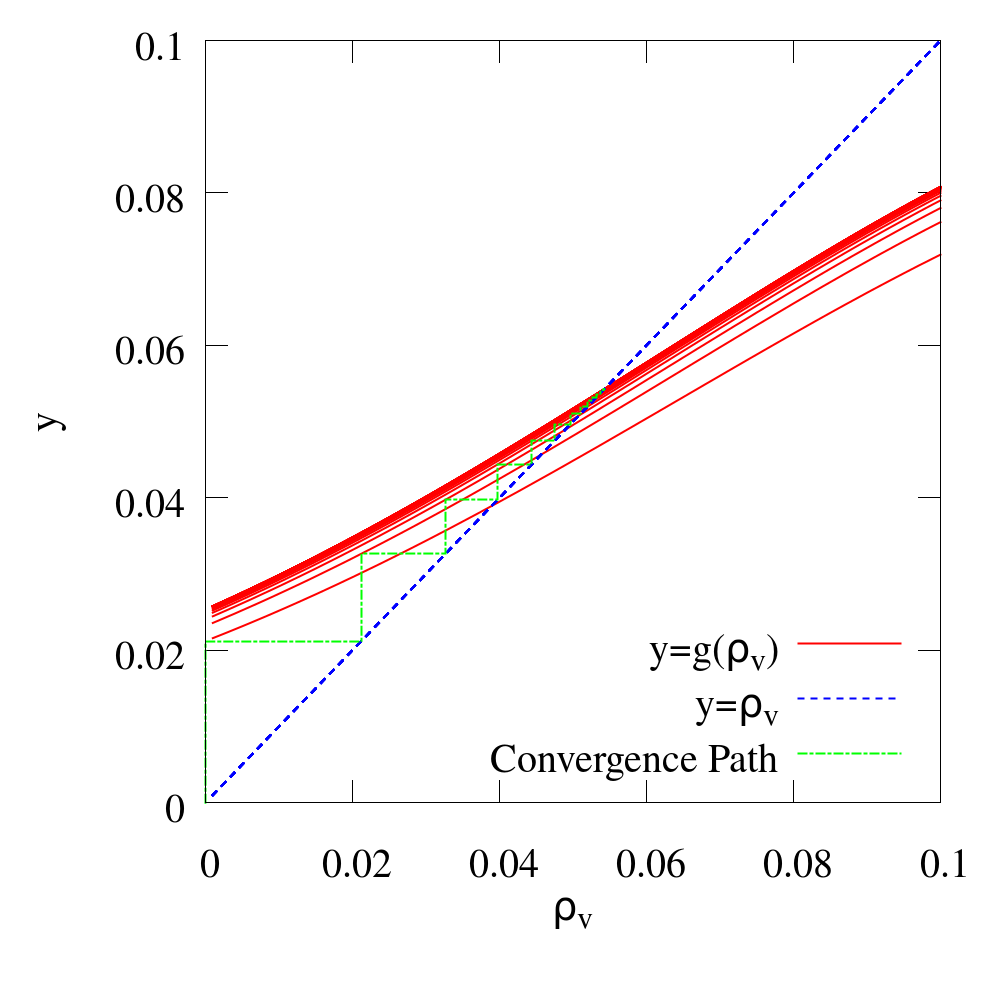
\includegraphics[scale=0.22]{Figures/NIST-VAL_FTT_C12_conv_0_42690.png}}
\subfloat[]{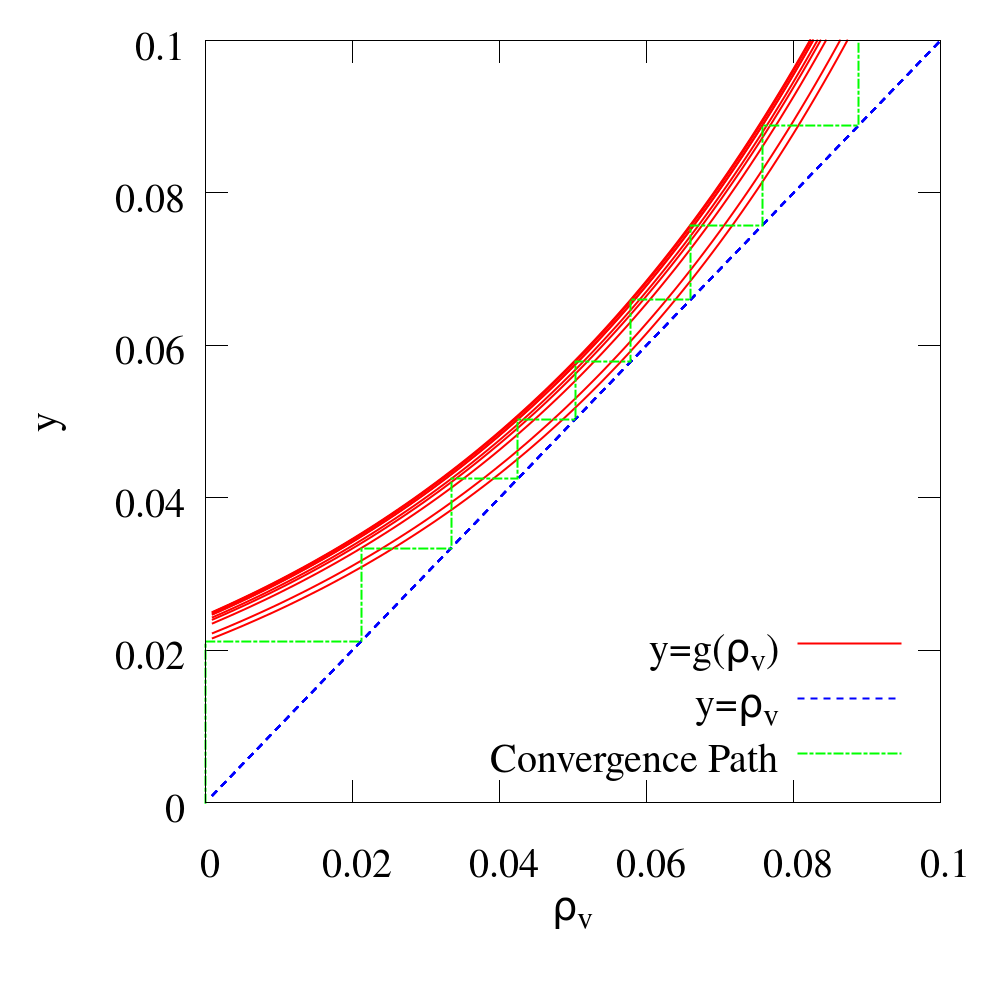
\includegraphics[scale=0.22]{Figures/NIST-VAL_FTF_C12_conv_0_42690.png}}
\caption{
Fixed-point method iteration and convergence path for \textit{n}-dodecane for the isochore corresponding to $\rho_{\mathrm{liq}}=0.4269\,\mathrm{g/cm^3}$. Eq.~(\ref{eqn:rhoV}) is summarized into $\rho_{\mathrm{vap}}=g(\rho_{\mathrm{vap}})$, i.e. the standard form of fixed-point method, where the $g(\rho_{\mathrm{vap}})$ curves represent the right-hand side of Eq.~(\ref{eqn:rhoV}). At each iteration, $g(\rho_{\mathrm{vap}})$ is calculated based on a new set of $T^{\mathrm{sat}}$, $P^{\mathrm{sat}}$, $A^\mathrm{dep}$, and $Z_{\mathrm{liq}}$. Iteration starts with a low initial guess for $\rho_{\mathrm{vap}}$ and stops when absolute percent deviation between two consecutive $\rho_{\mathrm{vap}}$ values is less than a small tolerance, e.g. 0.1 \%.
The blue line represents the 45-degree line. \textbf{a)} $B_3$ term is used in Eq.~(\ref{eqn:eqn11})
, \textbf{b)} $B_3$ term is excluded from Eq.~(\ref{eqn:eqn11}). Using $B_3$ helps iteration to converge for high $T^{\mathrm{sat}}$ values.}
\label{fig:convergence-path}
\end{figure*}

\subsection{Vapor Pressure Sensitivity to Virial Coefficients} \label{sec:Bx-Sensitivity}
In this section, we investigate the sensitivity of vapor pressure to accuracy of $B_2$ and $B_3$ at saturation temperatures as well as $B_2$ at supercritical isothermal temperature. This is important because $B_2$ and $B_3$ are often unknown for a given force field. 

In order to estimate the required accuracy of the second virial coefficient at the isothermal temperature, Figure~\ref{fig:B2-sensitivity}(a) is generated by changing the REFPROP $B_2$ and calculating the corresponding deviations in \textit{n}-dodecane vapor pressure. For example, a 5 \% change in $B_2$ results in around 2 \% deviation in \textit{n}-dodecane $P^{\mathrm{sat}}$. This shows that it is imperative to use an accurate $B_2$ value at the isothermal temperature.

Vapor pressure estimate is very weakly influenced at low saturation temperatures by accuracy of the second and third virial coefficients in Eq.~(\ref{eqn:rhoV}) and Eq.~(\ref{eqn:psat}). Figure~\ref{fig:B2-sensitivity}(b) shows the $P^{\mathrm{sat}}$ sensitivity to $B_2$ at various reduced temperatures, each representing one isochore. The first three lowest temperatures, are fairly insensitive to $B_2$ precision such that even 50 \% error in $B_2$ results in less than 1 \% deviation in $P^{\mathrm{sat}}$. However, a relatively accurate $B_2$ is required to obtain accurate $P^{\mathrm{sat}}$ when $T_\mathrm{r}^\mathrm{sat}>0.75$. Similarly, when $T_\mathrm{r}^\mathrm{sat} \approx 0.84$ $B_2$ deviations must not be greater than 2 \% in order to have less than 1 \% error in vapor pressure.

Figure~\ref{fig:B2-sensitivity}(c) was plotted similar to Figure~\ref{fig:B2-sensitivity}(b), with respect to $B_3$. It is worth mentioning that in order to truly understand the influence of $B_3$, exact values of $B_2$ were used from NIST REFPROP. Even though adding $B_3$ improves the overall behavior of fixed-point iteration in terms of convergence (Figure~\ref{fig:convergence-path}), the sensitivity of $P^{\mathrm{sat}}$ to $B_3$ is negligible when $T_\mathrm{r}^\mathrm{sat}$ is less than 0.85. This supports the idea of setting the $B_3$ term to zero without significant loss of precision at such temperatures. 

Similar to Figure~\ref{fig:B2-sensitivity}, the effect of changing virial coefficients on $\rho_\mathrm{vap}$ and $T^\mathrm{sat}$ was considered. The sensitivity of $\rho_\mathrm{vap}$ to virial coefficients is similar to $P^\mathrm{sat}$, and $T^\mathrm{sat}$ was found to be insensitive to virial coefficient deviations.

\begin{figure*}
\centering
\subfloat[]{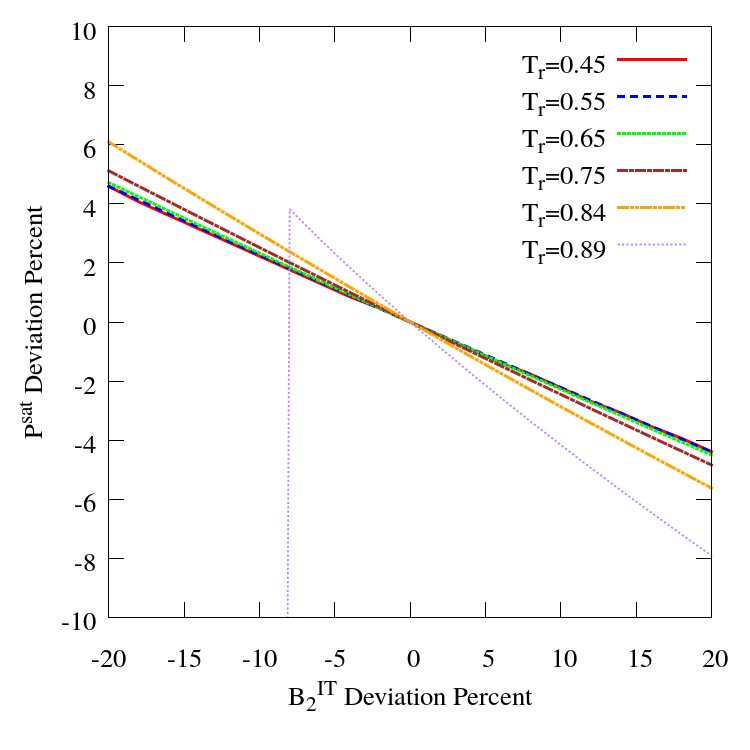
\includegraphics[scale=0.22]{Figures/FTF-B2xX-IT-C12-Psat.png}}
\subfloat[]{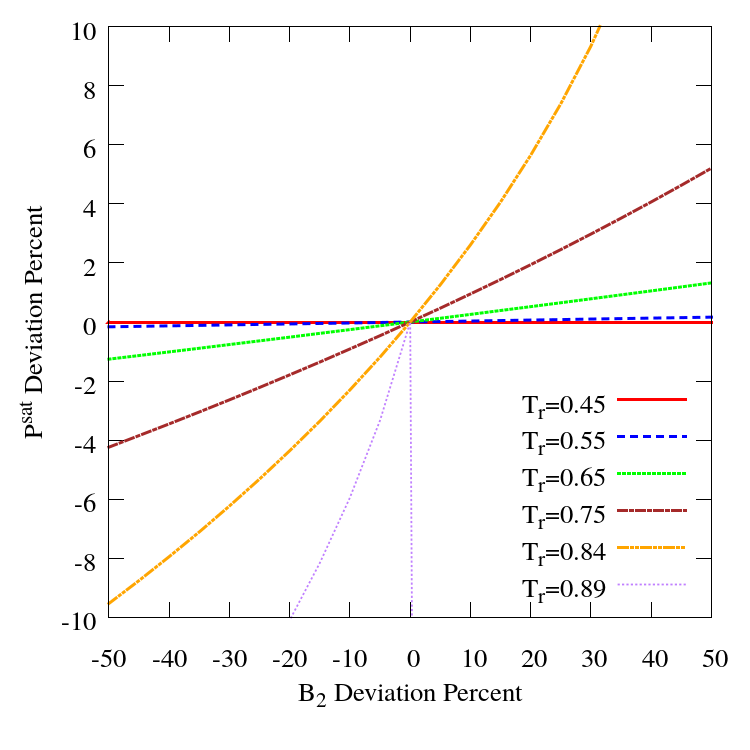
\includegraphics[scale=0.22]{Figures/FTF-B2xX-C12-Psat.png}}
\subfloat[]{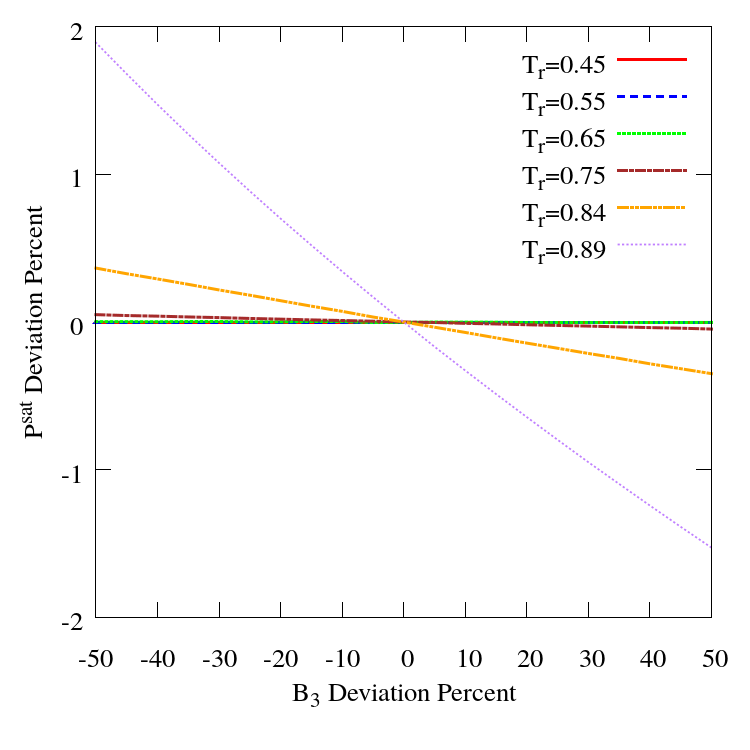
\includegraphics[scale=0.22]{Figures/FTT-B3xX-C12-Psat.png}}
\caption{
\textbf{a)} \textit{n}-Dodecane $P^{\mathrm{sat}}$ sensitivity to isotherm $B_2$
,\textbf{b)} $P^{\mathrm{sat}}$ sensitivity to second virial coefficient used in Eq.~(\ref{eqn:psat})
, and \textbf{c)} $P^{\mathrm{sat}}$ sensitivity to third virial coefficient used in Eq.~(\ref{eqn:psat})
}
\label{fig:B2-sensitivity}
\end{figure*}

\begin{figure*}
\centering
\subfloat[]{\includegraphics[scale=0.22]{Figures/NisVal-Deviation-Psat.png}}
\subfloat[]{\includegraphics[scale=0.22]{Figures/NisVal-Deviation-rhoL.png}}
\subfloat[]{\includegraphics[scale=0.22]{Figures/NisVal-Deviation-rhoV.png}}
\caption{
Sensitivity of the ITIC method to $T^\mathrm{sat}_\mathrm{est}$ for \textit{n}-dodecane. The ITIC method is applied using REFPROP values of $Z$ and $U^\mathrm{dep}$. The y-axis represents percent deviation of the corresponding property calculated using ITIC compared with REFPROP saturation data. Triangles pointing up or down represent ITIC results when $T^\mathrm{sat}_\mathrm{est}$ is increased or decreased by the percentage shown in the legend, respectively. $B_3$ is not included in Eq.~(\ref{eqn:rhoV}).
}
\label{fig:Nist-val-tsat-sensitivity}
\end{figure*}

\subsection{Sensitivity to Estimated Saturation Temperature} \label{sec:tsat-sensitivity}
As mentioned in Section~\ref{sec:ITIC-method}, saturation liquid densities in the ITIC method are fixed values at which we compute other saturation properties. This requires an initial estimate for saturation temperatures at the densities of interest.
 
It is important that the ITIC method does not depend strongly on the accuracy of $T^\mathrm{sat}_\mathrm{est}$. Figure~\ref{fig:Nist-val-tsat-sensitivity} demonstrates that deviations in $P^\mathrm{sat}$ are less than 1 \% and deviations in $\rho_\mathrm{liq}$ are less than 0.25 \% when errors in $T^\mathrm{sat}_\mathrm{est}$ are within 10 \%. Deviations in $\rho_\mathrm{vap}$ are less than 1 \%, except for the high temperature point for which deviations are smaller than 3 \%. This can be improved by including $B_3$. Typical errors in $T^\mathrm{sat}_\mathrm{est}$ are less than 1 \%, in which case the deviations for all three properties are nearly indistinguishable from the deviations resulting from numerical integration alone, i.e., those for 0 \% error in $T^\mathrm{sat}_\mathrm{est}$. 

Note that in Figure~\ref{fig:Nist-val-tsat-sensitivity}, isochoric/isothermal properties ($Z$ and $U^\mathrm{dep}$) used for determining saturation properties are obtained from REFPROP. If $T^\mathrm{sat}_\mathrm{est}$ percent deviation shown in the legend of Figure~\ref{fig:Nist-val-tsat-sensitivity}(a) is less than zero (i.e. $T^\mathrm{sat}_\mathrm{est} < T^\mathrm{sat}_\mathrm{REFPROP}$), some of the ITIC points are in metastable state. Since the REFPROP database does not provide $Z$ and $U^\mathrm{dep}$ for such points, a linear extrapolation of REFPROP data was used to approximate $Z$ and $U^\mathrm{dep}$. A similar sensitivity analysis using simulation results is included in supplementary material.

\section{Simulation Details} \label{sec:SimDetail}
In principle, both Monte Carlo and molecular dynamics methods can be used to simulate the $NVT$ state points required to construct the isothermal and isochoric paths in the ITIC method. In this study, the MC method with fixed bond lengths is favored due to smaller uncertainties at low density. The Cassandra \cite{Shah2017} and GOMC (GPU Optimized Monte Carlo) \cite{Mick2013} packages are used to simulate several molecules in $NVT$ ensemble using united-atom potential models. In united-atom force fields, interaction sites may consist of a group of atoms, which is centered on the main atom of the group for the TraPPE-UA method \cite{Smit1998}. In the TraPPE-UA model van der Waals interactions are truncated at $1.4\,\mathrm{nm}$ and standard analytical long-range corrections are applied to compensate for truncation effects on energy and pressure\cite{allen2017}. Furthermore, the bond lengths are considered fixed and the bond energy is zero. This approximation results in smaller pressure fluctuations at low densities, but we note that the MC results at high densities were consistent with MD results simulated in Large-scale Atomic/Molecular Massively Parallel Simulator (LAMMPS) \cite{Plimpton2007} and GROMACS \cite{Lindahl2001} within their uncertainties.

For each compound, 26 $NVT$ points are simulated in order to obtain 5 saturation points, as illustrated in Figure~\ref{fig:ITICpathway}. The density of the isochore with highest density is chosen to match the experimental liquid density at the minimum reduced saturation temperature ($T_\mathrm{r}^\mathrm{min}$) of 0.45. Densities and temperatures of all simulated state points are listed in the supplementary material along with average pressures and average energies.

The Packmol \cite{martinez2009packmol} software is used to create the initial configurations for LAMMPS and GOMC simulations, while Cassandra simulations were initialized using internal capabilities of this software. The simulation boxes contain 1200 sites except for the four simulations required for estimating $B_2$ at the isotherm temperature (the purple and green diamonds in Figure~\ref{fig:ITICpathway}) for which simulation boxes contain 4800 sites. Standard Periodic Boundary Conditions (PBCs) are used. Simulations are run for 10 million Monte Carlo steps, and the last 5 million MC steps are used for calculating the properties which ar stored every 50,000 MC steps. 


In order to approximate the computational cost of the ITIC method, \textit{n}-dodecane  coexistence points obtained at reduced temperatures of 0.65, 0.75, and 0.85 using  GEMC are compared with the ITIC coexistence points obtained at liquid densities corresponding to reduced temperatures of approximately 0.65, 0.75, and 0.85. This temperature range is chosen because both  GEMC and ITIC are reliable within $0.65<T_\mathrm{r}<0.85$. Cassandra package is used for both simulations using an AMD 1.3 GHz processor. 3,500 and 13,500 MC cycles are used for equilibration and production of GEMC simulation, using five block averages to characterize the uncertainty. The average run-time of the three GEMC simulations is 15.8 hours with each simulation running on a separate CPU core, resulting in an average $P^\mathrm{sat}$ uncertainty of 7.5 \% (relative standard error). On the other hand, running ITIC state points for 500 MC cycles of equilibration and 2000 MC cycles of production with four block averages reproduced the GEMC results with 7.1 \% $P^\mathrm{sat}$ uncertainty. The ITIC simulations were run on 20 CPU core. The maximum run-time (highest density and lowest temperature) of ITIC simulations is 18.9 hours. Therefore, when the number of available CPU cores is not limited, the ITIC method is approximately 20\% slower than GEMC. If ITIC coexistence points at reduced temperatures of 0.45 and 0.55 are to be included, the maximum run-time slightly increases (i.e. 22.3 hours $\approx$ 40 \% additional computational time compared to GEMC), whereas GEMC is not feasible for \textit{n}-dodecane, unless a thermodynamic integration approach (i.e. Gibbs-Duhem) is used to extend the lower temperature limit of GEMC.

%If ITIC coexistence points at reduced temperatures of 0.45 and 0.55 are to be included, the maximum run-time slightly increases (i.e. 22.3 hours $\approx$ 40 \% additional computational time compared to GEMC), whereas GEMC is not feasible for \textit{n}-dodecane.

\subsection{Internal Energy Departure Function Calculation}\label{sec:udepCalc}
The internal energy departure function in Eq.~(\ref{eqn:eqn8}) can be calculated for isochoric points using Eq.~(\ref{eqn:uDepForm})

\begin{equation}
U^{\mathrm{dep}} = \frac{E^{\mathrm{tot}} - E^{\mathrm{bonded}} - E^{\mathrm{intra}}}{NRT}\label{eqn:uDepForm}
\end{equation}
where $E^{\mathrm{tot}}$, $E^{\mathrm{bonded}}$, and $E^{\mathrm{intra}}$ are the total potential energy, bonded energy (bond, angle, and dihedral), and intramolecular pairwise energy (coulumbic and van der Waals). Failing to subtract $E^{\mathrm{intra}}$ causes a significant error in vapor pressure. A post-processing code is required to calculate this quantity, if the molecular simulation package does not provide an internal way of estimating $E^{\mathrm{intra}}$. For example, LAMMPS simulations require this post-processing.  In this case it is necessary to output the site coordinates periodically after the simulation reaches equilibrium. 

An underlying assumption of Eq.~(\ref{eqn:eqn8}) is that the intramolecular energy (ideal gas contribution) does not depend on density of the system. This assumption might not hold true for dense systems and large molecules, where the overall configuration of moleucles, hence the intramolecular non-bonded and bonded energies, is affected by closeness of the molecules. A more rigorous way of calculating ideal gas energy is to obtain the total energy from simulation of a single molecule system. 

%Todo: In Section~\ref{sec:ExampleSim}, we confirm that $U^\mathrm{dep}$ values from Eq.~(\ref{eqn:eqn8}) and single molecule approach are in agreement within their uncertainties.

\subsection{Bootstrapping Method for Uncertainty Calculation}\label{sec:bootstrapping}
Bootstrapping is used to estimate the statistical uncertainties \cite{Efron1981} in $T^\mathrm{sat}$, $P^\mathrm{sat}$, $\rho_\mathrm{vap}$, and $\Delta H_\mathrm{v}$. Note that the ITIC method determines saturation conditions at a fixed value of $\rho_{\mathrm{liq}}$ (equal to the isochoric density) and, therefore, the bootstrap uncertainty in $\rho_{\mathrm{liq}}$ is zero. Four series of independent $NVT$ simulations are performed for each compound using different random number generator seeds. Each series of $NVT$ simulations comprises 26 state points including four at $T_\mathrm{r}=0.9$ and three on isotherm used to estimate $B_2$. ITIC analysis is performed using $NVT$ state points randomly selected from the four series, and saturation properties are computed. This process is repeated 500 times resulting in 500 sample values for each saturation property. The standard deviations are then calculated from the resulting 500 ITIC outputs. 

The resulting uncertainties are used to generate error bars represented in Figure~\ref{fig:EXAMPLE-SIM/all}, however in most cases the error bars are smaller than the symbols. For greater clarity, uncertainties are tabulated in supplementary material for each property at each saturation condition.

\section{Calculation of Virial Coefficients} \label{sec:VirialCalc}
Mayer Sampling is a common approach for estimating virial coefficients of a given force field \cite{singh2004mayer}. For example, Kofke and Schultz implement this approach for \textit{n}-alkanes \cite{Schultz2010a}. Efforts like those of Kofke and Schultz could make simulations on the lower end of supercritical isotherm unnecessary \cite{barlow2015communication}, in addition to facilitating computations just below the critical temperature.  Furthermore, the higher virial coefficients play a significant role on their own merits in the development of high accuracy equations of state for simulation models \cite{thol2016equation}.

In this study, we use a simpler approach that is amenable for developing a correlation for $B_2$ and $B_3$ with respect to temperature. Second virial coefficients are estimated by calculating the intercept of $(Z-1)/\rho$ with respect to $\rho$. In principle, the slope of this line at zero density also gives the third virial coefficient. Figure~\ref{fig:TraPPE-C2-Z1rho-B2-B3} shows the accuracy of this method when used at various temperatures. The blue lines in Figure~\ref{fig:TraPPE-C2-Z1rho-B2-B3}(a) are obtained from Eq.~(\ref{eqn:Z1rhoB2B3})

\begin{equation}
\frac{Z-1}{\rho} = B_2 + B_3\rho \label{eqn:Z1rhoB2B3}
\end{equation}
where the intercept ($B_2$) and slope ($B_3$) correspond to Schultz's values \cite{Schultz2010a}.

Figure~\ref{fig:TraPPE-C2-Z1rho-B2-B3}(a) shows that for TraPPE-UA ethane at temperatures above $T_\mathrm{r}^{\mathrm{sat}}=0.85$, $B_2$ values calculated using this method agree with values reported by Schultz to within 2 \%. In Figure~\ref{fig:TraPPE-C2-Z1rho-B2-B3}(a), $Z$ at $T_\mathrm{r} = 0.8$ and $\rho \approx 0.085\,\mathrm{g/cm^3}$ is not consistent with the Schultz values due to proximity with the two-phase region. Therefore, using the lowest three densities would give a more accurate estimate for those temperatures. It is worth considering that the value of accurate virial coefficient characterization is enhanced in the context of the ITIC method.  

\begin{figure*}
\centering
\subfloat[]{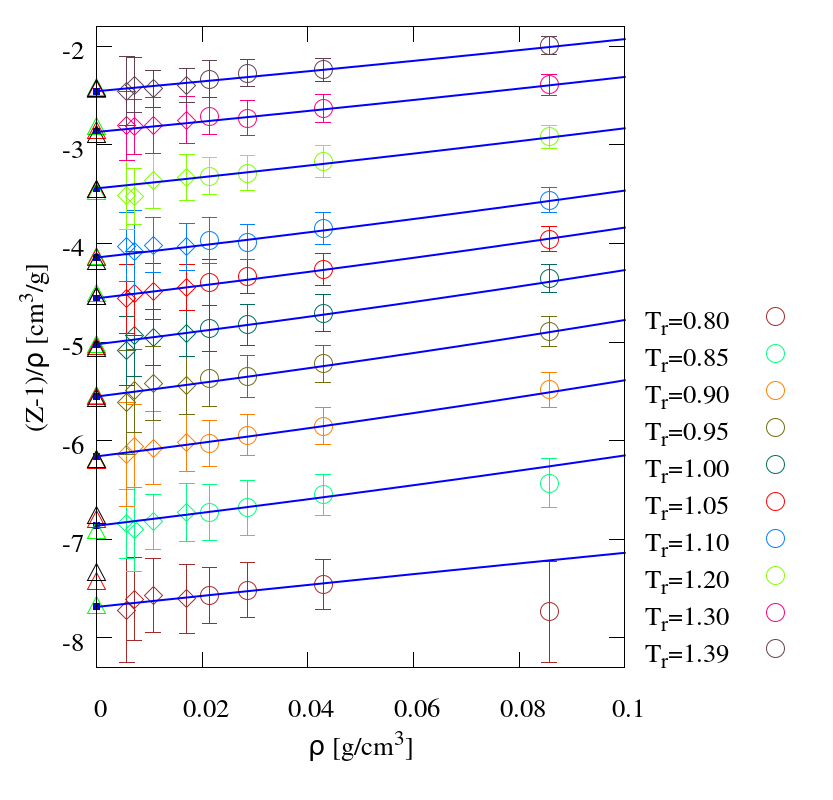
\includegraphics[scale=0.20]{Figures/TraPPE-C2-Z1rho.png}}
\subfloat[]{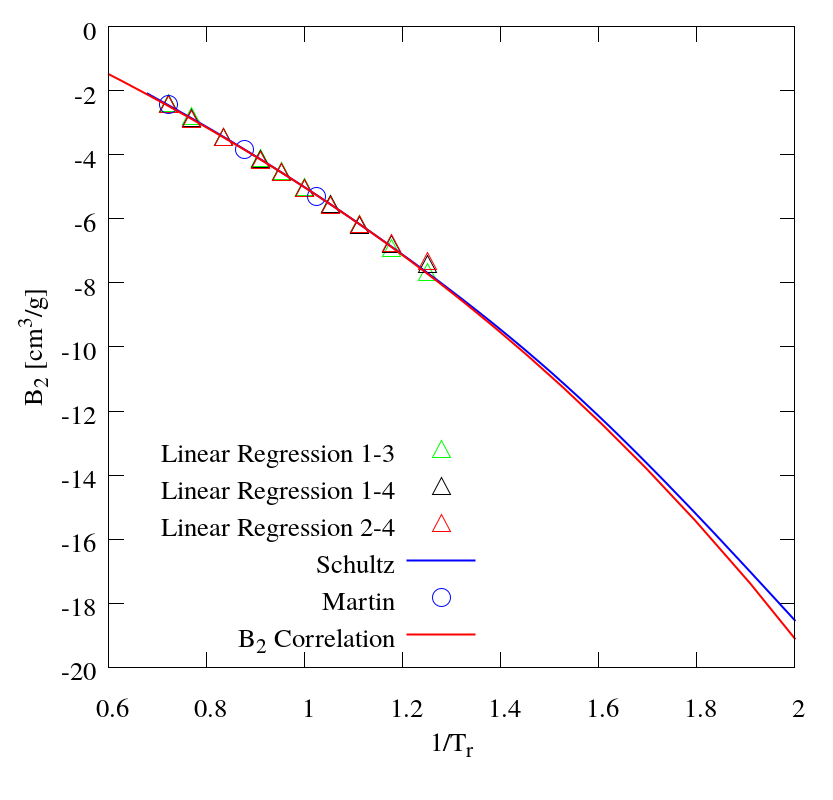
\includegraphics[scale=0.20]{Figures/TraPPE-C2-B2.png}}
\subfloat[]{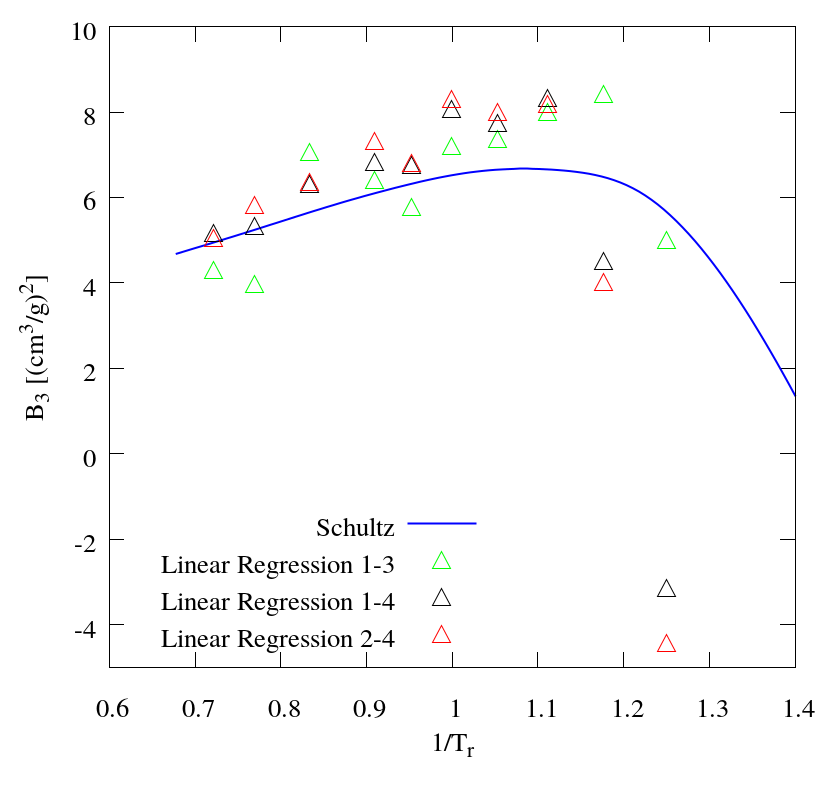
\includegraphics[scale=0.20]{Figures/TraPPE-C2-B3.png}}
\caption{
Panel \textbf{a)} shows the plot of $(Z-1)/\rho$ with respect to $\rho$ for TraPPE-UA ethane. Blue solid squares represent Schultz's $B_2$ values.~\cite{Schultz2010a}. Blue dashed lines represent Schultz values of $B_2$ (intercept) and $B_3$ (slope). Circles and diamonds are $NVT$ state points simulated with the GOMC package \cite{Mick2013}. Using circles in a) suffices to obtain accurate virial coefficients, therefore diamond points are are not used in $B_2$ and $B_3$ calculations. In panel \textbf{b)} and \textbf{c)} black squares represent the median of $B_2$ and $B_3$ when circle points \{1,2,3\}, \{1,2,3,4\}, \{2,3,4\}, and \{1,2,4\} from panel \textbf{a)} were used in linear regression according to Eq.(\ref{eqn:Z1rhoB2B3}). Error bars represent bootstrapped uncertainties. The blue circles in panel \textbf{b)} represent $B_2$ values obtained by Martin and Siepmann \cite{Martin1998} using a Monte Carlo method \cite{Harismiadis1994}.
}
\label{fig:TraPPE-C2-Z1rho-B2-B3}
\end{figure*}

According to Eq.~(\ref{eqn:rhoV}), it is important to have a correlation for $B_2$ and $B_3$ with respect to temperature, because $T^\mathrm{sat}$ estimates change after each iteration and updated values for $B_2$ and $B_3$ are needed. Recently, a Taylor Series expansion with Mayer Sampling approach has been utilized to generate correlations with respect to temperature for $B_2$ and $B_3$ \cite{Hatch2017}. In this study, we obtain such a correlation from the formula used in the DIPPR \cite{DIPPR2004} database, except the last term is omitted to decrease the number of parameters and avoid overfitting, as shown in Eq.~(\ref{eqn:b2form}) 

\begin{equation}
B_2=A+\frac{B}{T}+\frac{C}{T^3} \label{eqn:b2form}
\end{equation}

Eq.~(\ref{eqn:b2it}) and Eq.~(\ref{eqn:b2TrPoint9}) are obtained by inserting $B_2$ values extrapolated using Eq.~(\ref{eqn:Z1rhoB2B3}) and their corresponding temperatures into Eq.~(\ref{eqn:b2form}). 

\begin{equation}
B_2(T_{\mathrm{IT}})=A+\frac{B}{T_{\mathrm{IT}}}+\frac{C}{T_{\mathrm{IT}}^3} \label{eqn:b2it}
\end{equation}

\begin{equation}
B_2(T_{0.9})=A+\frac{B}{T_{0.9}}+\frac{C}{T_{0.9}^3} \label{eqn:b2TrPoint9}
\end{equation}
where $T_{0.9}$ is the temperature corresponding to reduced temperature of 0.9 and $T_\mathrm{IT}$ represents the isothermal temperature. 

Subtracting Eq.~(\ref{eqn:b2TrPoint9}) from Eq.~(\ref{eqn:b2it}) gives


\begin{equation}
B_2(T_{\mathrm{IT}})-B_2(T_{0.9})=B \left( \frac{1}{T_{\mathrm{IT}}}-\frac{1}{T_{0.9}} \right) +C \left( \frac{1}{T_{\mathrm{IT}}^3}-\frac{1}{T_{0.9}^3} \right) \label{eqn:b2subtract}
\end{equation}

Taking the derivative of $B_2$ with respect to $\beta$, as shown in Eq.~(\ref{eqn:dB2dbeta}) leads to the internal energy departure function

\begin{equation}
\rho \frac{\beta \partial B_2}{\partial \beta}=\rho \left( \frac{B}{T}+\frac{3C}{T^3}\right)=\frac{U-U_\mathrm{ig}}{RT} \label{eqn:b2uDep}
\end{equation}

Therefore, the intercept of $\frac{U-U_\mathrm{ig}}{\rho RT}$ with respect to $\rho$ gives the value of $\beta \frac{\partial B_2}{\partial \beta}$. Having this value can lead to Eq.~(\ref{eqn:b2pB2pBeta}) with two unknowns ($B$ and $C$)

\begin{equation}
\beta \frac{\partial B_2}{\partial \beta}=\frac{B}{T_{0.9}}+\frac{3C}{T_{0.9}^3} \label{eqn:b2pB2pBeta}
\end{equation}

Solving three equations (Eq.~(\ref{eqn:b2it})/(\ref{eqn:b2TrPoint9}), (\ref{eqn:b2subtract}), and (\ref{eqn:b2pB2pBeta})) with three unknowns gives the values of A, B, and C, hence a correlation for $B_2$ with respect to temperature is derived. Figure~\ref{fig:TraPPE-C2-Z1rho-B2-B3}(b) shows a correlation obtained by this method which is in good agreement with Schultz's simulation results \cite{Schultz2010a}.

$B_3$ calculation using Eq.~(\ref{eqn:Z1rhoB2B3}) deviates significantly from the rigorous values, as shown in Figure~\ref{fig:TraPPE-C2-Z1rho-B2-B3}(c). Therefore, $B_3$ values estimated this way are useful but should be regarded as ``effective" values that indirectly account for $B_4$ and higher order terms. On the other hand, more accurate representation of $(Z-1)/\rho$ is achieved using the $B_3^\mathrm{eff}$ from Eq.~(\ref{eqn:Z1rhoB2B3}) than using the rigorous $B_3$ or the rigorous $B_3$ and $B_4$ in combination, as shown in Figure~\ref{fig:FSE_TraPPE_C2_abc} (compare solid and dashed black lines with green line). Note that in the ITIC applications considered in this study, only second virial coefficient is used, therefore obtaining accurate $B_3$ is not a concern.

%For the current implementation of ITIC, Eq.~(\ref{eqn:Z1rhoB2B3}) with $B_3^\mathrm{eff}$ is used at $T_\mathrm{r}^\mathrm{sat} > 0.85$.

\section{Finite Size Effects}\label{sec:FSE}
According to Figure~\ref{fig:B2-sensitivity}(a), $P^{\mathrm{sat}}$ accuracy is sensitive to accuracy of $B_2$ values at the isothermal temperature ($B_2^{\mathrm{IT}}$). This sensitivity is due to accumulation of errors when integrating along isotherm, such that an error in $B_2^{\mathrm{IT}}$ affects the $A^{\mathrm{dep}}$ values at all other points along the isotherm and isochores. Similarly, one would expect a significant influence from low density points, i.e. points 1, 2, and 3 in Figure~(\ref{fig:ITICpathway}). Therefore, it is important to investigate the factors affecting the accuracy of $Z$ at low densities on the isotherm. The factors considered in this study are system size, the choice of MD or MC, and the choice of fixed bonds or flexible bonds. 

The system size effects at low densities are demonstrated in Figure~\ref{fig:FSE_TraPPE_C2_abc}. Plot of $(Z-1)/\rho$ with respect to $\rho$ shown in Figure~\ref{fig:FSE_TraPPE_C2_abc}(a) demonstrates the effect of varying number of molecules in MD simulation of ethane with rigid bonds. In order to match the $B_2+B_3 \rho+B_4 \rho^2$ line which represents the rigorous values of $(Z-1)/\rho$, we need 3200 ethane molecules to achieve low enough uncertainties for accurate extrapolation of $B_2$ for the simulation times chosen. In the MD simulations shown in Figure~\ref{fig:FSE_TraPPE_C2_abc}(a) C-C bonds are held constant using the SHAKE algorithm \cite{Ryckaert1977}. 

The effect of using flexible bonds is shown in Figure~\ref{fig:FSE_TraPPE_C2_abc}(b). The systematic discrepancy from rigorous values (solid black line) as well as large uncertainties suggests not using flexible bonds at very low densities. A major problem with MD simulations with flexible bonds is the large pressure and energy fluctuations leading to the need for long equilibration and production times.


Figure~\ref{fig:FSE_TraPPE_C2_abc}(c) shows the low density $NVT$ state points simulated using GOMC \cite{Mick2013}. This plot shows that the MC method gives more reliable results than MD for low density $NVT$ state points. 

Table~\ref{tab:FSE} compares the uncertainties of $Z$ when using different simulation methods. $\mathrm{STD}_1$ represents the average of four relative standard deviations of $Z$ (i.e., $\mathrm{STD}/Z\times100 \, \%$), each calculated during a single run, while $\mathrm{STD}_2$ is the relative standard deviation of $Z$ from four separate runs. According to this table, the standard deviations from four replicate simulations ($\mathrm{STD}_2$) are much smaller than the average standard deviation for a single run ($\mathrm{STD}_1$). Therefore, Figure~\ref{fig:FSE_TraPPE_C2_abc} is plotted based on $\mathrm{STD}_2$ uncertainties. Table~\ref{tab:FSE} also shows that MC results have nearly an order of magnitude smaller $\mathrm{STD}_1$ and $\mathrm{STD}_2$ than rigid or flexible MD results when $N < 3200$.  

Therefore, we recommend using MC when simulating these low density points. The choice of MD or MC for other high density state points in ITIC method is less important, because they generally agree with each other within their uncertainties. In this study, we use MC for all state points when computing VLE.

\begin{table*}[]
\centering
\caption{Compressibility factor and uncertainty at low densities. $\mathrm{STD}_1$ represents the average of four relative standard deviations each calculated during the corresponding individual runs, while $\mathrm{STD}_2$ is the relative standard deviation of $Z$ from four separate runs.}
\label{tab:FSE}
%%%\begin{ruledtabular}
\begin{tabular}{cc|cc|cc|cc|cc}
       &        & \multicolumn{2}{c}{N=120} & \multicolumn{2}{c}{N=400} & \multicolumn{2}{c}{N=1600} & \multicolumn{2}{c}{N=3200} \\
Method & $\rho [\mathrm{g/cm^3}]$ & $\mathrm{STD}_1 \%$  & $\mathrm{STD}_2 \%$ & $\mathrm{STD}_1 \%$  & $\mathrm{STD}_2 \%$ & $\mathrm{STD}_1 \%$  & $\mathrm{STD}_2 \%$  & $\mathrm{STD}_1 \%$  & $\mathrm{STD}_2 \%$ \\
\hline
MC-rigid    & 0.0214 & 1.05   & 0.10 & 0.62   & 0.05 & 0.46  & 0.05 & -     & -    \\
MC-rigid    & 0.0286 & 1.27   & 0.11 & 0.69   & 0.06 & 0.55  & 0.06 & -     & -    \\
MC-rigid    & 0.0429 & 1.60   & 0.17 & 0.96   & 0.00 & 0.76  & 0.11 & -     & -    \\
MC-rigid    & 0.0857 & 2.54   & 0.23 & 1.59   & 0.08 & 1.38  & 0.17 & -     & -    \\
MC-rigid    & 0.1714 & 4.54   & 0.26 & 3.16   & 0.26 & 2.91  & 0.30 & -     & -    \\
MC-rigid    & 0.2571 & 6.55   & 0.60 & 4.62   & 0.63 & 4.32  & 0.25 & -     & -    \\
\hline
MD-rigid    & 0.0214 & 11.71  & 0.94 & 6.31   & 0.72 & 3.20  & 2.41 & 2.30  & 0.10 \\
MD-rigid    & 0.0286 & 13.56  & 1.02 & 7.33   & 0.16 & 3.80  & 4.78 & 2.60  & 0.11 \\
MD-rigid    & 0.0429 & 17.30  & 0.76 & 9.46   & 0.53 & 4.79  & 2.45 & 3.23  & 0.20 \\
MD-rigid    & 0.0857 & 28.35  & 1.14 & 15.01  & 0.36 & 7.49  & 0.39 & 5.15  & 0.36 \\
MD-rigid    & 0.1714 & 49.89  & 1.53 & 25.46  & 1.73 & 13.56 & 0.55 & 9.15  & 0.64 \\
MD-rigid    & 0.2571 & 65.65  & 2.44 & 35.96  & 0.75 & 18.38 & 0.52 & 12.57 & 0.47 \\
\hline
MD-flexible & 0.0214 & 106.25 & 1.39 & 59.51  & 0.88 & 29.67 & 0.78 & 19.12 & 0.56 \\
MD-flexible & 0.0286 & 113.52 & 2.01 & 61.35  & 0.45 & 30.83 & 0.66 & 20.39 & 0.59 \\
MD-flexible & 0.0429 & 129.34 & 3.16 & 65.61  & 0.71 & 35.84 & 0.32 & 22.10 & 0.34 \\
MD-flexible & 0.0857 & 152.29 & 2.52 & 83.85  & 1.15 & 42.60 & 1.20 & 27.49 & 0.33 \\
MD-flexible & 0.1714 & 196.67 & 2.49 & 101.51 & 2.90 & 53.94 & 0.82 & 38.10 & 0.46 \\
MD-flexible & 0.2571 & 227.96 & 0.94 & 125.42 & 1.28 & 58.77 & 1.60 & 42.61 & 0.87
\end{tabular}
%\end{ruledtabular}

\end{table*}

\begin{figure*}
\centering
\subfloat[MD rigid]{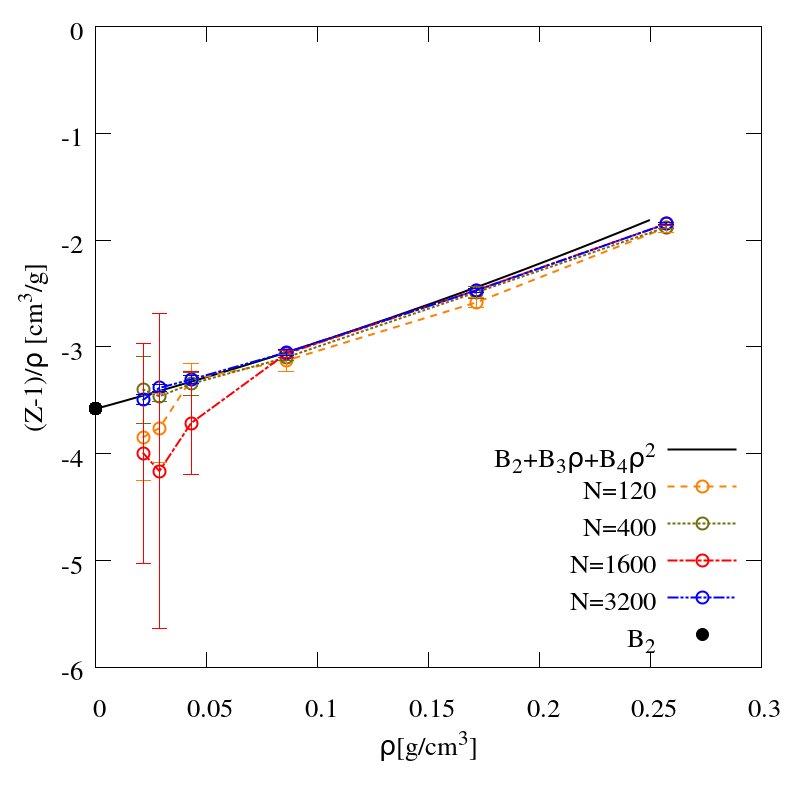
\includegraphics[scale=0.22]{Figures/FSE_TraPPE-C2_Lammps-rigid_IT.png}}
\subfloat[MD flexible]{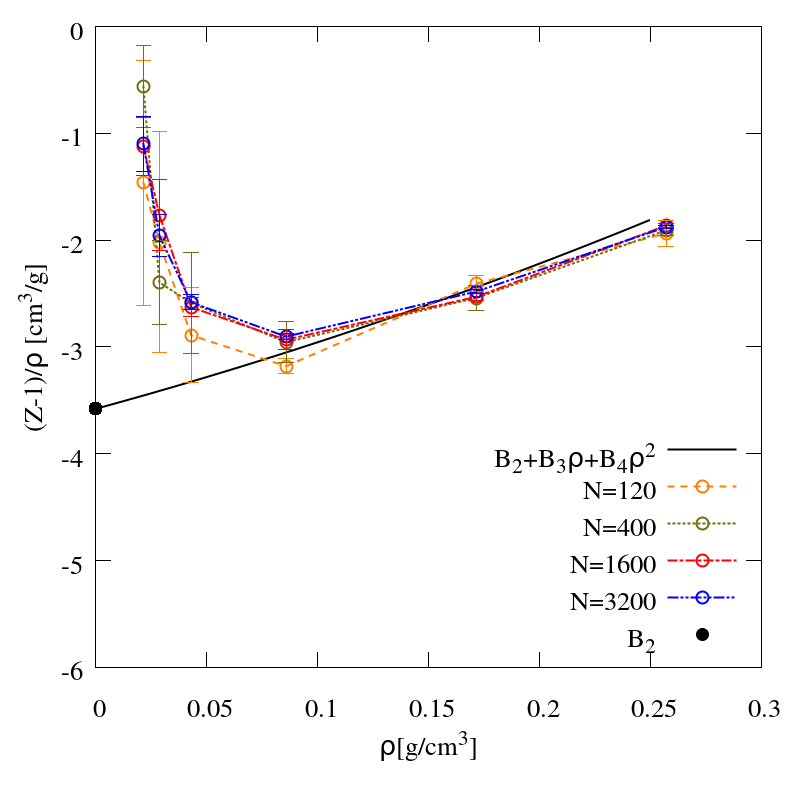
\includegraphics[scale=0.22]{Figures/FSE_TraPPE-C2_Lammps-flex_IT.png}}
\subfloat[MC rigid]{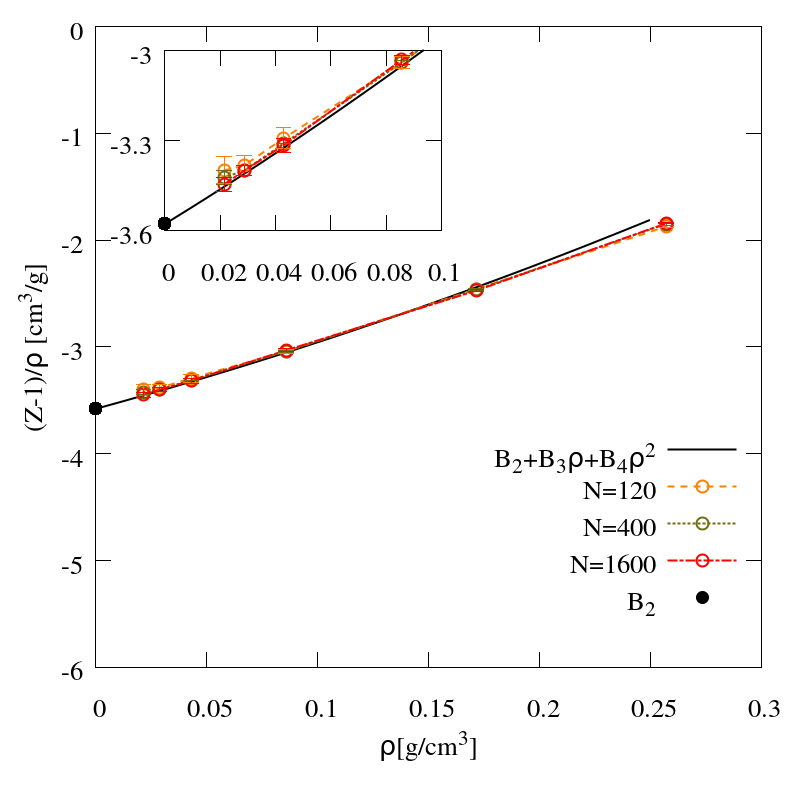
\includegraphics[scale=0.22]{Figures/FSE_TraPPE-C2_GOMC_IT.png}}
\caption{ Effect of number of ethane molecules on compressibility factor at low densities at $T^{\mathrm{IT}}=360$. Panel \textbf{a)} is from MD with rigid bonds (using SHAKE algorithm in LAMMPS), panel \textbf{b)} is from MD with flexible bonds (harmonic potential using multiple-time-step algorithm RESPA \cite{tuckerman1992} algorithm), and panel \textbf{c)} is from MC with rigid bonds (GOMC). 
Solid black lines represent $B_2+B_3 \rho+B_4 \rho^2$ curve where $B_{2-4}$ are obtained from Schultz's work \cite{Schultz2010a}. Dashed black lines represent $B_2+B_3 \rho$ line where $B_{2-3}$ are obtained from Schultz's work. Solid black circle shows the Schultz's value of $B_2$. Dashed green lines represent $B_2+B_3^\mathrm{eff}rho$ where $B_2$ and $B_3^\mathrm{eff}$ are fit to four lowest density simulation values. Note that the increasing  deviation between black line and simulation points at higher densities is due to truncation of virial equation at $B_4$. The error bars illustrate the standard deviation calculated based on four separate runs with different initial configurations.
}
\label{fig:FSE_TraPPE_C2_abc}
\end{figure*}

\begin{figure*}[]
\subfloat[]{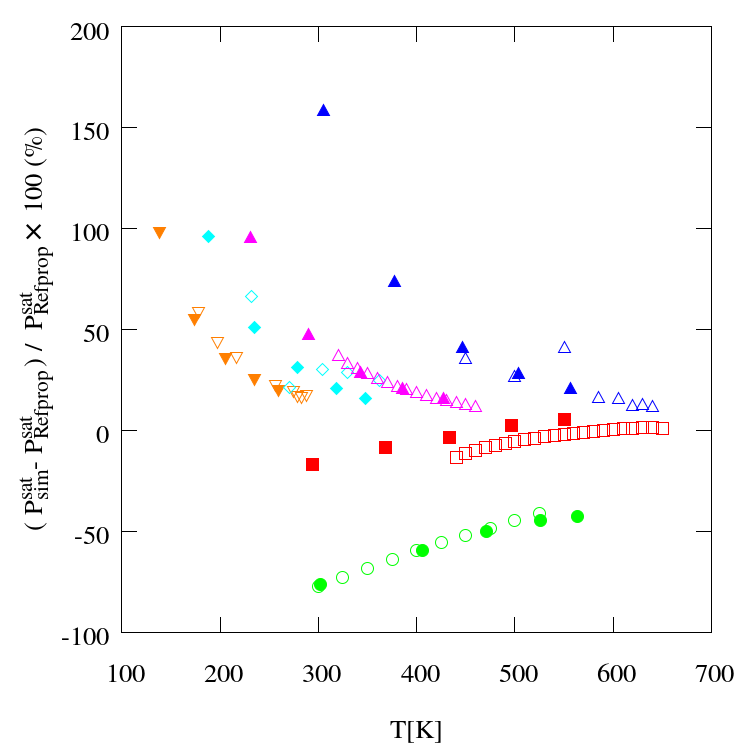
\includegraphics[scale=0.23]{Figures/Deviation-Psat.png}}
\subfloat[]{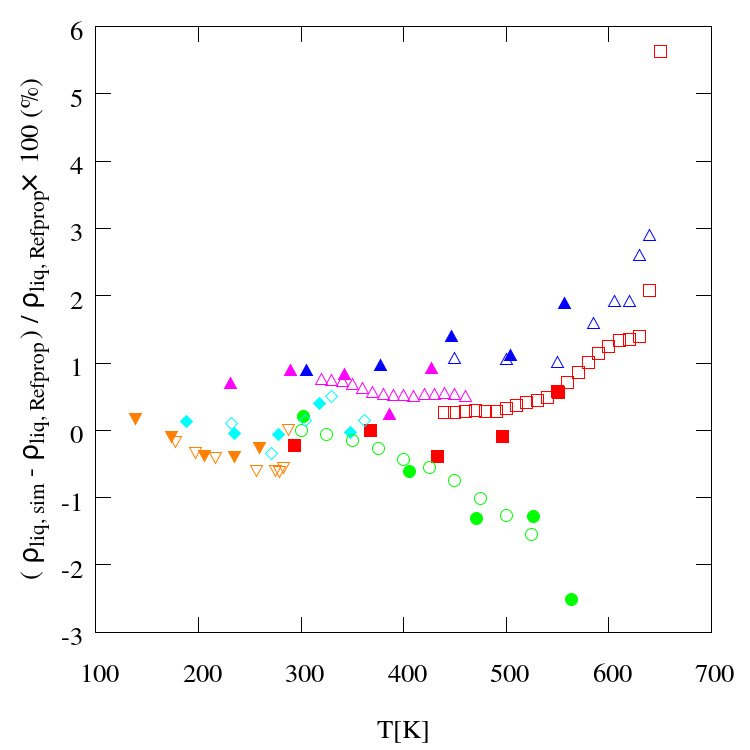
\includegraphics[scale=0.23]{Figures/Deviation-rhoL.png}}
\subfloat[]{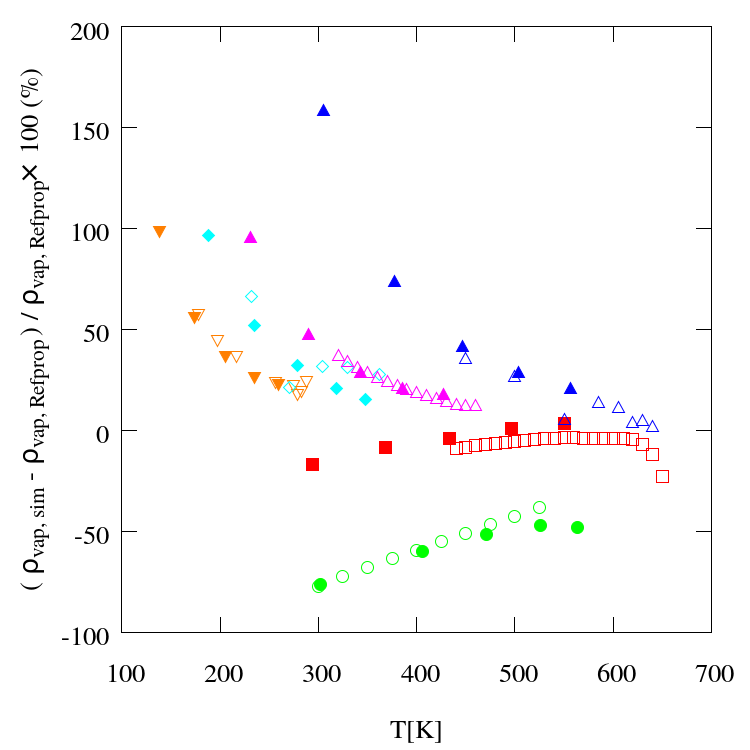
\includegraphics[scale=0.23]{Figures/Deviation-rhoV.png}}
\caption{Comparison between ITIC (filled) with respect to GEMC and GCMC methods (unfilled). The y-axis represents deviation from REFPROP data. 
GEMC: TraPPE-UA \textit{n}-dodecane  (orange) \cite{Martin1998}, TraPPE-UA ethane (cyan) \cite{Martin1998}, TraPPE-UA isobutane (purple) \cite{Wick2000};
GCMC: TraPPE methane\cite{Shen2008} (blue), Mie-UA \textit{n}-dodecane (red) \cite{Potoff2009}, TIP4P/2005 water (green) \cite{Shen2008}, and TraPPE-UA isohexane (brown) \cite{Mick2017}. Black filled symbols represent ITIC results simulated with GROMACS \cite{Lindahl2001}. Black unfilled triangles represent TraPPE-UA \textit{n}-dodecane from Ref.~\cite{Ungerer2000}.
%Todo: Fix deviation plots
% -The liquid density results for MieC12 and isobutane look very bad. Is there some way to clean this up
% -add percent deviation values between ITIC and MC for Fig 9 in discussion
}
\label{fig:EXAMPLE-SIM/Deviation-Psat-rhoL-rhoV}
\end{figure*}

\begin{figure*}[]
\centering
\subfloat[]{\includegraphics[scale=0.30]{Figures/EXAMPLE-SIM_GEMC_psat.png}}\label{aa}
\subfloat[]{\includegraphics[scale=0.30]{Figures/EXAMPLE-SIM_GEMC_trho.png}}\label{bb}\\
\subfloat[]{\includegraphics[scale=0.30]{Figures/EXAMPLE-SIM_GCMC_psat.png}}\label{cc}
\subfloat[]{\includegraphics[scale=0.30]{Figures/EXAMPLE-SIM_GCMC_trho.png}}\label{dd}
\caption{
Comparison between ITIC method and Monte Carlo methods: GEMC (TraPPE-UA \textit{n}-dodecane \cite{Martin1998}, TraPPE-UA ethane \cite{Martin1998}, and TraPPE-UA isobutane \cite{Wick2000}), and GCMC (TraPPE-UA methane \cite{Shen2008}, Mie-UA \textit{n}-dodecane \cite{Potoff2009}, TIP4P/2005 water \cite{Shen2008}, and TraPPE-UA isohexane \cite{Mick2017}). $B_2$ values at saturation temperatures were obtained using low density simulations described in Section~\ref{sec:VirialCalc}, except for TIP4P/2005 simulation where $B_2$ correlation is obtained from Ref.~\cite{Benjamin2007,Chialvo2006}.
}
\label{fig:EXAMPLE-SIM/all}
\end{figure*}

\section{Example Simulations} \label{sec:ExampleSim}
The TraPPE-UA \cite{Martin1998,Martin1999,Wick2000}, Mie-UA \cite{Potoff2009,Mick2017,Barhaghi2017,Mick2015}, and TIP4P/2005 \cite{Abascal2005} models were chosen for the purpose of testing the ITIC method due to the availability of literature vapor-liquid coexistence simulation results. Figures ~\ref{fig:EXAMPLE-SIM/Deviation-Psat-rhoL-rhoV} and \ref{fig:EXAMPLE-SIM/all} demonstrate good agreement between traditional GEMC/GCMC methods and the ITIC approach using both MC and MD.

Figure~\ref{fig:EXAMPLE-SIM/Deviation-Psat-rhoL-rhoV} provides a quantitative comparison between ITIC method and traditional vapor-liquid coexistence Monte Carlo methods. In this figure deviation of ITIC and MC methods from REFPROP data are compared. Figure~\ref{fig:EXAMPLE-SIM/all} shows the Clausius-Clapeyron and coexistence curves for all example simulations compared to MC methods. In all ITIC calculations, $B_2$ is included in Eq.~(\ref{eqn:rhoV}) and Eq.~(\ref{eqn:psat}), while $B_3$ is set to zero for simplicity. Initial $T^\mathrm{sat}$ values for all the compounds shown in Figures ~\ref{fig:EXAMPLE-SIM/Deviation-Psat-rhoL-rhoV} and \ref{fig:EXAMPLE-SIM/all} are obtained from DIPPR \cite{DIPPR2004} database. Complete information about chosen ITIC state points as well as the results of $NVT$ simulations is included in Supplementary Materials.

Saturation points calculated using the ITIC method are compared against TraPPE-UA results obtained using GEMC which are available from the TraPPE website \cite{eggimann2014}. Figure~ \ref{fig:EXAMPLE-SIM/Deviation-Psat-rhoL-rhoV}, \ref{fig:EXAMPLE-SIM/all}(a), and \ref{fig:EXAMPLE-SIM/all}(b) compare the ITIC and GEMC results for pure ethane, \textit{n}-dodecane, and isobutane systems. $NVT$ simulations at ITIC state points are performed using the Cassandra Monte Carlo \cite{Shah2017} and GROMACS molecular dynamics \cite{Lindahl2001} packages. 

The ITIC method was also compared to histogram-reweighting GCMC provided in Figure~\ref{fig:EXAMPLE-SIM/all}(c) and Figure~\ref{fig:EXAMPLE-SIM/all}(d). GCMC results for Mie-UA \textit{n}-dodecane are not available below a minimum reduced temperature ($T_\mathrm{r}^{\mathrm{min}}$) of 0.67, however the ITIC method allowed us to calculate vapor pressure and liquid densities for reduced temperatures as low as 0.45. 

In order to validate the ITIC method for polar molecules, the results of the ITIC method using TIP4P/2005 water simulated in Cassandra were compared against TIP4P/2005 data from the NIST Standard Reference Simulation Website \cite{Shen2008} simulated using grand-canonical Wang-Landau/Transition-matrix Monte Carlo and histogram re-weighting. Figure~ \ref{fig:EXAMPLE-SIM/Deviation-Psat-rhoL-rhoV}, \ref{fig:EXAMPLE-SIM/all}(c), and \ref{fig:EXAMPLE-SIM/all}(d) show the agreement between the two methods for TIP4P/2005 water. The absolute average percent deviation between vapor pressure calculated using ITIC method and GCMC method for TIP4P/2005 water shown in Figure~ \ref{fig:EXAMPLE-SIM/Deviation-Psat-rhoL-rhoV}(a) is less than 1 \%.

 The isothermal/isochoric plots of Helmholtz energy departure function, compressibility factor, and internal energy departure function as well as plots of second virial coefficient and heat of vaporization for all example simulations are included in supplementary material. Also included in supplementary material are tables containing ITIC results for all example simulations.

Figure~\ref{fig:EXAMPLE-SIM/all} includes the critical points obtained using the method described in Section~\ref{sec:ITIC-method}. The ITIC coexistence points 
shown in this figure do not exceed $T_\mathrm{r}^\mathrm{sat} \approx 0.85$, the estimated critical properties are subject to larger uncertainties and possible systematic deviations. In the case of TIP4P/2005 water, critical point calculation requires a more suitable method as shown in Ref.~\cite{Vega2006}.

%Prerev: Figure~\ref{fig:EXAMPLE-SIM/all} includes the critical points obtained using the method described in Section~\ref{sec:ITIC-method}. Even though the ITIC coexistence points shown in this figure do not exceed $T_\mathrm{r}^\mathrm{sat} \approx 0.85$, acceptable critical properties were obtained, with the exception of TIP4P/2005 water. A more suitable method has been used in Ref.~\cite{Vega2006} to calculate critical properties of water.

One limitation of the ITIC approach is the need for a reasonable value of $T_\mathrm{est}^\mathrm{sat}$. The ITIC calculations shown so far are done for well-known molecules for which extensive experimental data are available. All force fields considered (TraPPE-UA, Mie-UA, TIP4P/2005) provide accurate representation of the $T^\mathrm{sat}$ vs. $\rho_\mathrm{liq}$ curve compared to experimental data. Therefore, the $T_\mathrm{est}^\mathrm{sat}$ values for these compounds were obtained from DIPPR database. However, it is important to make sure that ITIC method also works for the molecules for which experimental data are not available. For example, 1-naphthalenyl, 4-phenanthrenyl butane is a large aromatic with 5 rings and 28 united-atom sites for which,to the best of our knowledge, no experimental data is available. In this case, a simple linear extrapolation using two points (red (x) symbols in Figure~\ref{fig:Ex_Sim_TraPPE-1p4nB}(a)) along the isochore is used to obtain $T_\mathrm{est}^\mathrm{sat}$, i.e. the temperature at which $Z\approx0$. Once $T_\mathrm{est}^\mathrm{sat}$ is calculated, the procedure in Figure~2 is followed. Figure~\ref{fig:Ex_Sim_TraPPE-1p4nB}(b-c) shows a good agreement between the ITIC method with GEMC results.

Alternatively, one can improve ITIC results by running the ITIC procedure iteratively by using $T\mathrm{sat}$ from the previous iteration. It's worth mentioning that we do not need to resimulate the isotherms, and the isochoric information from previous iterations can potentially help improve the integration accuracy along the isochores. 



\begin{figure*}[]
\centering
\subfloat[]{\includegraphics[scale=0.20]{Figures/Ex_Sim_TraPPE-1p4nB_zt.png}}\label{cc}
\subfloat[]{\includegraphics[scale=0.20]{Figures/Ex_Sim_TraPPE-1p4nB_psat.png}}\label{aa}
\subfloat[]{\includegraphics[scale=0.20]{Figures/Ex_Sim_TraPPE-1p4nB_trho.png}}\label{bb}
\caption{
Simulation of 1-naphthalenyl,4-phenanthrenyl butane based on an extended TraPPE-UA model \cite{Yiannourakou2018}. Both ITIC and GEMC results are obtained using GOMC. Red (x) symbols are simulated at two arbitrarily chosen temperatures to obtain $T_\mathrm{est}^\mathrm{sat}$ for each isochore. 
}
\label{fig:Ex_Sim_TraPPE-1p4nB}
\end{figure*}

\section{Conclusions} \label{sec:conclusion} 
The ITIC method is shown to be a reliable alternative for phase equilibrium calculations. In the absence of simulation uncertainty, the vapor pressure calculated by the ITIC method with 9 points on isotherm and 3 points on isochore reproduces NIST REFPROP vapor pressure within 1 \% deviation. In applications where simulation uncertainty is significant, ITIC is sensitive to low density $NVT$ simulations, but the noise at low densities can be addressed by simulating larger systems, and preferring $NVT$ Monte Carlo method with fixed bond lengths when feasible.

It is important for engineering applications to be able to simulate systems at temperatures as low as $T_\mathrm{r}=0.45$. Monte Carlo methods such as GEMC and GCMC usually have a minimum reduced temperature limit of about 0.6, due to the insertion/transfer moves The ITIC method, hence, outperforms GEMC and GCMC when $T_\mathrm{r}$ is less than 0.6. This method, on the other hand, is less favorable at high reduced temperatures, especially above $T_\mathrm{r}=0.85$, mostly due to lack of a convenient method to characterize the virial coefficients. In addition, ITIC requires high temperature high pressure property estimates, which provide additional information for force field characterization.

In conclusion, ITIC can easily be implemented from $T_\mathrm{r} = 0.45$ to $0.85$ with approximately 40 \% additional computational time over the 0.6 to 0.85 temperature range using GEMC. If temperatures above 0.85 are required, it is recommended to approach the problem of coexistence calculation with a combination of Monte Carlo (GEMC or GCMC) and isothermal-isochoric integration. If a single method is preferred, or if MD is the preferred simulation method, ITIC has notable advantages. These advantages could be enhanced over time with the availability of rigorous higher order virial coefficients for broader ranges of molecular types. 

\section{Acknowledgments}

This research was performed while R.A.M. held a National Research Council (NRC) Postdoctoral Research Associateship at the National Institute of Standards and Technology (NIST). Contribution of NIST, an agency of the United States government; not subject to copyright in the United States.
%%%

\section{Supplementary Material} \label{sec:SupMat} 
See supplementary material for 
%density, temperature, compressibility factor, and energies of simulated state points for all simulated compounds, as well as 
the isothermal/isochoric plots of $A^{\mathrm{dep}}$, $U^{\mathrm{dep}}$, $Z$, and plots of $\Delta H_{\mathrm{v}}$, and $B_2$ for all example simulations. Also included are data shown in Figure~\ref{fig:Nist-Val-Deviation} and figures of $T^\mathrm{sat}_\mathrm{est}$ sensitivity study using simulation data.
\section{References} \label{sec:ref} 

%\section*{References}

\bibliography{ITIC-Paper}

\end{document}
